\documentclass[12pt,letterpaper,ngerman]{article}
%\usepackage[letterpaper,top=3.0cm, bottom=3.0cm, footnotesep=1.0cm]{geometry}
\usepackage[letterpaper,margin=1in]{geometry} % e. Set margins of 1 inch (2.54 cm.) on all four sides of the paper. 
\usepackage{mathptmx} % d. ...in a simple roman face except where indicated below (§3). 
\usepackage[singlespacing]{setspace} % Set line spacing to 1 throughout the document
\usepackage{fancyhdr} 

% Set the headheight to at least 14.49998pt
\setlength{\headheight}{14.49998pt}

% Optionally adjust \topmargin if necessary
% \addtolength{\topmargin}{-2.49998pt}
\usepackage{relsize}

\usepackage[bottom]{footmisc}
\usepackage{tabularx}
    
\pagestyle{empty}        % No page numbers

% Set paragraph indentation to 1.5cm
\setlength{\parindent}{2em}

%%%Using XeTeX (xelatex, lulatex):
%\usepackage{polyglossia}
%\usepackage{fontspec}
%\usepackage{xunicode}
%\usepackage{xltxtra}
\usepackage{url}
\usepackage{hyperref}
\usepackage[english,german]{babel}

\usepackage{graphicx}

%\setmainfont[Mapping=tex-text]{Linux Libertine O} %Falls nicht vorhanden müssen die LinLibertine-ttf-Dateien nach C:\windows\fonts verschoben werden

\usepackage{booktabs}    % For nice-looking tables
\usepackage{natbib}      % Citation support (required for crossrefs)
\usepackage{expex}
\bibpunct[:]{(}{)}{;}{a}{}{,} % Defaults for in-text citations
\usepackage{bibentry}    % Print individual references

\usepackage{acronym}
\usepackage{multicol}

% TODO: set authors name
%vorgelegt von\\
%Name des Verfassers/der Verfasserin\\
\author{Author's name}

\usepackage{scrhack} % Recommended to avoid potential conflicts
\usepackage{microtype}

\usepackage[acronym,xindy,toc]{glossaries} % TODO: include "acronym" if glossary and acronym should be separated
\makeglossaries
\loadglsentries{pages/glossary.tex} % important update for glossaries, before document

\usepackage{ragged2e}

% Set up hyphenation rules for the language package when mistakes happen
\babelhyphenation[english]{
an-oth-er
ex-am-ple
}

\usepackage{enumitem}
\usepackage{babel}
\usepackage{pgfplots}
\usepackage{tikz}
\usepackage{minted}
\usepackage{subcaption}
\usepackage{physics}
\pgfplotsset{compat=1.18}
\usepgfplotslibrary{colormaps}
\usepgfplotslibrary{groupplots}
\usepgfplotslibrary{external} 
\tikzexternalize
\usepackage{graphicx}
\usepackage{epstopdf}
\usepackage{mathtools}
\usepackage{amssymb}
\usepackage{amsmath}
\usepackage{chngcntr}
\usepackage{float}
\usepackage{svg}
\usepackage{xcolor}
\usepackage{cite}
\usepackage{bookmark}
\usepackage{csquotes}
\MakeOuterQuote{"}
\usetikzlibrary{
  decorations.pathmorphing,
  automata, positioning, arrows, matrix,
  decorations.pathreplacing,
  shapes.geometric, calc,shapes.misc,
  arrows.meta,backgrounds,fit,petri
}
\pgfmathsetseed{\number\pdfrandomseed} % to ensure that it is randomized
\begin{document}
\DeclarePairedDelimiter\ceil{\lceil}{\rceil}
\DeclarePairedDelimiter\floor{\lfloor}{\rfloor}
\newcommand{\rand}[2]{
\pgfmathsetmacro{\thenum}{rand(0,1)}
\thenum
}
\newcommand{\nat}[0]{\mathbf{N}}
\newtheorem{example}{Beispiel}[section]
\newcommand{\mycomment}[1]{}


\definecolor{SkyBlue}{RGB}{135, 206, 235}
\definecolor{CrimsonRed}{RGB}{220, 20, 60}
\definecolor{ForestGreen}{RGB}{34, 139, 34}
\definecolor{Goldenrod}{RGB}{218, 165, 32}
\definecolor{DeepPurple}{RGB}{75, 0, 130}
\definecolor{Coral}{RGB}{255, 127, 80}
\definecolor{Teal}{RGB}{0, 128, 128}
\definecolor{Lavender}{RGB}{230, 230, 250}
\definecolor{Amber}{RGB}{255, 191, 0}
\definecolor{SlateGray}{RGB}{112, 128, 144}

\definecolor{ContrastRed}{RGB}{230, 25, 75}   % Red
\definecolor{ContrastGreen}{RGB}{60, 180, 75}   % Green 
\definecolor{ContrastBlue}{RGB}{0, 130, 200}   % Blue
\definecolor{ContrastOrange}{RGB}{245, 130, 48}  % Orange
\definecolor{ContrastPurple}{RGB}{145, 30, 180}  % Purple
\definecolor{ContrastCyan}{RGB}{70, 240, 240}  % Cyan
\definecolor{ContrastMagenta}{RGB}{240, 50, 230}  % Magenta
\definecolor{ContrastLime}{RGB}{210, 245, 60}  % Lime
\definecolor{ContrastPink}{RGB}{250, 190, 190} % Pink


\begin{center}\uppercase{Ludwig-Maximilians-Universität München}\end{center}
\begin{center}
  \uppercase{Programming languages and artificial intelligence}
\end{center}

\vspace*{10mm}
\begin{center}

\includegraphics[height=40mm]{abb/sigillum.png}
\end{center}
\vspace*{10mm}

\title{Titel der Arbeit}
\date{\vspace{-5ex}}
{\let\newpage\relax\maketitle}
\thispagestyle{empty}
\begin{center}
\begin{large}
\begin{Large}
Bachelorarbeit
\end{Large}
im Studiengang 'Informatik plus Mathematik' 
\end{large}
\end{center}
\vspace{1cm}
\begin{center}
\begin{large}
Betreuer: Prof. Dr. Johannes Kinder
\end{large}
\end{center}
\begin{center}
\begin{large}
Mentor: Moritz Dannehl, M.Sc.
\end{large}
\end{center}


\begin{center}
\begin{large}
Ablieferungstermin: \date{\today} 
\end{large}
\end{center}

\vspace{1,5cm}
\newpage \hfill\\
{\bf \Large Zusammenfassung}\\\\
In den letzten Jahren wurden große Fortschritte bei der Codierung von 
natürlichen Sprachen in reellwertigen Vektoren (engl. Embeddings) erzielt.
Diese Arbeit baut auf diesen Fortschritten auf, um aus den 
Informationen einer C-Quellcode-Funktion einen reellwertigen 
Vektor zu produzieren,
welcher den Inhalt der Funktion codiert. Diese Vektoren können dann 
verwendet werden, um ein neuronales Netzwerk mittels überwachten Lernens 
darauf zu trainieren, bei gegebener Funktion in Maschinensprache einen 
Vektor vorherzusagen, der den Inhalt der Funktion widerspiegelt. 
Die Embeddings werden zum einen aus Funktionsnamen, Funktionskommentaren 
und Code-Llama-Erklärungen \cite{rozière2024codellamaopenfoundation} 
erstellt, indem der rohe Text, mittels \textit{SentenceTransfomer} 
\cite{reimers-2019-sentence-bert} in einen Vektor umgewandelt wird.
Zum anderen wurden Inferenz-Vektoren aus dem 
\textit{Code2Vec} \cite{code2vec} Modell verwendet.  
Um die Qualität der Code-Llama-Vektoren, \textit{Code2Vec}-Vektoren, 
Funktionskommentar-Vektoren und Funktionsnamen-Vektoren einzuordnen,
wurden sie qualitativ und quantitativ verglichen. Zunächst wurde die 
beste Methode mittels einer Expertenbefragung identifiziert.  
Dabei stellte sich heraus, dass Code Llama die besten Embeddings 
produziert. Danach wurden die \textit{Code2Vec}-Vektoren, 
Funktionskommentar-Vektoren und Funktionsnamen-Vektoren quantitativ 
mittels einer Formel mit den Code-Llama-Vektoren verglichen. 
Schließlich wurden die Code-Llama-Vektoren, \textit{Code2Vec}-Vektoren,
Funktionskommentar-Vektoren und Funktionsnamen-Vektoren qualitativ
mittels \textit{t-SNE} auf Gruppierungen untersucht. Nach
qualitativer 
und quantitativer Auswertung konnten die Embeddings 
absteigend nach Qualität folgendermaßen angeordnet werden:
Code-Llama-Vektoren, Funktionsnamen-Vektoren, 
Funktionskommentare-Vektoren und \textit{Code2Vec}-Vektoren.
\\\\
{\bf \Large Abstract}\\\\
In recent years, there have been great advances in encoding 
natural languages in real-valued vectors. This  progress can
be used to generate embeddings out of natural language 
information in C source code. These embeddings can then be 
used to train a neural network with supervised learning.
Given a function in binary code, this neural network
predicts a vector that reflects the content of the function.
These embeddings are generated by the \textit{SentenceTransformer}
\cite{reimers-2019-sentence-bert}
using function names, function comments and Code Llama 
\cite{rozière2024codellamaopenfoundation}
explanations.
In addition, we compare embeddings generated by the \textit{Code2Vec}
\cite{code2vec}
model.To classify the quality of Code Llama vectors,
\textit{Code2Vec} vectors, function comment vectors 
and function name vectors, they were compared qualitatively
and quantitatively.
The best method was identified through an expert survey.  
It was found that Code Llama produced the best embeddings. 
The \textit{Code2Vec} vectors, function comment vectors and
function name vectors were compared quantitatively with the
Code Llama vectors using a formula. 
Finally, the Code Llama, \textit{Code2Vec},  function comment 
and function name vectors were 
compared qualitatively using \textit{t-SNE}. 
After qualitative and quantitative evaluation, the embeddings can 
be ranked in descending order of quality as follows: 
Code llama vectors, function name vectors, function comment vectors 
and \textit{Code2Vec} vectors.
\newpage
\tableofcontents
\newpage

\setcounter{page}{1}
\pagestyle{fancy}
\fancyhf{}
\counterwithin{figure}{section}
\fancyhead[R]{\thepage}
\renewcommand{\headrulewidth}{0pt} %obere Trennlinie
\newtheorem{definition}{Definition}
\section{Einführung}
In den letzten Jahren wurden wichtige Fortschritte in der natürlichen
Sprachverarbeitung erzielt, ein wichtiger Faktor war die Codierung von
natürlicher Sprache in reellwertigen Vektoren (engl. embeddings). Die 
hochdimensionalen Vektoren
codieren die Semantik der ursprünglichen Wörter oder Sätze.
Diese hochdimensionalen Vektoren, die die Semantik von
Wörtern oder Sätzen codieren, erlauben es, neuronale
Netzwerke in diversen Anwendungsbereichen zu trainieren,
wie beispielsweise \textit{Spam Detection} \cite{Ball2019}.  
Zu den bekanntesten Modellen, die natürliche Sprache in Vektoren abbilden, gehören 
\textit{Word2Vec} \cite{word2vec},
\textit{WordPiece} \cite{wu2016googlesneuralmachinetranslation} und
\textit{SentenceTransformer} \cite{reimers-2019-sentence-bert}.\\
Diese Fortschritte in der natürlichen Sprachverarbeitung, indem
ein großer Faktor war, Wörter und Sätze in hochdimensionalen 
Vektoren zu codieren, dienen als Motivation auch 
Assembler-Quellcode in einem Vektor zu codieren, der den Inhalt
des Quellcodes widerspiegelt. Die resultierenden Vektoren, die 
den Inhalt des Binärcodes codieren, können dann wieder benutzt 
werden, um neuronale Netzwerke auf diverse Anwendungen zu 
trainieren, wie Beispielsweise
\textit{Binary Code-Similarity-Detection} \cite{jtrans},
\textit{Function-Boundary-Detection} \cite{190918},
\textit{Function-Type-Inference}\cite{203650},
\textit{Binary Code-Search} \cite{9345532},
Reverse Engineering \cite{reverse-engeneering},
oder das Klassifizieren von 
Maleware in der Maschinensprache\cite{maleware-detection}.\\
Um ein Modell mittels überwachten Lernens zu trainieren, das
Binärcode in Vektoren abbildet, welche den Inhalt des 
Binärcodes widerspiegelt, ist für jede Assembler-Funktion
ein Vektor erforderlich, der den Inhalt der Funktion codiert.
Dieser, für das überwachte Lernen erforderliche Datensatz,
kann aus C-Quellcode erzeugt werden, falls ein Tool vorliegt
welches aus C-Quellcode-Funktionen Vektoren generiert,
welche den Inhalt der Funktion widerspiegeln. Um schließlich 
noch die Binärcode-Funktionen zu erhalten, werden die 
C-Quellcode-Funktionen kompiliert.\\\\
\textit{Das Ziel dieser Arbeit} ist es, verschiedene Methoden 
zu vergleichen aus C-Quellcode, mithilfe von Werkzeugen 
aus der natürlichen Sprachverarbeitung, Vektoren zu generieren die 
den Inhalt des Quellcodes widerspiegeln.\\\\
Der Prozess des Kompilierens reduziert Funktionen
auf die für den Computer wesentlichsten Bausteine, dabei gehen viele 
Informationen verloren, wie Funktionsnamen, Variablennamen und
Kommentare. Diese Informationen sind von großer Bedeutung, da
sie Hinweise über die Funktionsweise und den Anwendungszweck der
Funktion geben. Durch die Verwendung dieser Informationen 
könnte der Inhalt des Quellcodes besser in einen Vektor codiert
werden.\\
Aufgrund der Tatsache, dass diese Informationen in der natürlichen 
Sprache sind, ist es sinnvoll, bewährte Werkzeuge aus der natürlichen 
Sprachverarbeitung zu verwenden, um diese in Vektoren zu codieren. 
Aus den resultierenden Vektoren kann schließlich ein Datensatz
generiert werden, der ein neuronales Netzwerk darauf trainiert, 
Binärcode als hochdimensionale, reellwertige Vektoren abzubilden,
die den Inhalt des Quellcodes codieren.
\pagebreak
\subsection{Stand der Technik}
{\bf CLAP} ({\bf C}ontrastive {\bf L}anguage {\bf A}ssembly 
{\bf P}re-training) von Wang et al.
setzte Anfang 2024 einen neuen Stand der Technik in
\textit{Binary Code-Simillarity-Detection}
mithilfe von natürlicher Sprachverarbeitung\cite{clap}.
Die Aufgabe bei 
\textit{Binary Code-Simillarity-Detection}
besteht darin, die Ähnlichkeit zwischen zwei gegebenen 
Assemblercodes zu bestimmen.\\
Das CLAP-Modell ist aus zwei Teilen zusammengesetzt: einem Assembler-Encoder 
und einem Text-Encoder. Der Assembler-Encoder, der aus Assemblercode 
reellwertige Vektoren erzeugt, knüpft mit kleinen Änderungen an den vorherigen
Stand der Technik von JTrans an. Der Text-Encoder ist eine neue Erweiterung,
die darauf abzielt, den Text wieder in einen reellwertigen Vektor zu 
konvertieren. Wang et al. starten dabei mit einem Modell aus der natürlichen 
Sprachverarbeitung namens \textit{SentenceTransformer} und trainieren dieses
darauf, Assemblercode die passende Quellcodeerklärung  zuzuordnen. Dabei 
erhalten sie die Quellcodeerklärungen durch ein Large  Language-Model, wie
beispielsweise Chat-GPT.\\
Das {\bf JTrans}-Modell \cite{jtrans} 
baut auf einer Modellarchitektur aus der natürlichen 
Sprachverarbeitung namens 
Transformer \cite{transformer} auf. 
Wang et. al behandeln die einzelnen Assembler-Instruktionen als Wörter, um so 
die Transformer-Modellarchitektur anwenden zu können. Außerdem codieren sie
Kontrollflussinformationen des Assembler-Codes in die Eingabe des 
Transformer-Modells. Mit diesem Ansatz erzielten sie im Jahre 2022 einen neuen
Stand der Technik in \textit{Binary Code Similarity Detection}.\\
\subsection{Ergebnisse der Arbeit}
Die hauptsächlichen Ergebnisse dieser Arbeit sind:
\begin{itemize}
  \item Ein Tool, das einen Datensatz mit Assemblercode und
    Vektoren, welche den Inhalt des Assemblercodes widerspiegeln,
    aus C-Quellcode und dem dazugehörigen Assemblercode generiert.
  \item Eine qualitative Analyse mithilfe von
    \textit{t-SNE} \cite{JMLR:v9:vandermaaten08a}, die die
    Gruppierung im 2-dimensionalen von 
    Funktionskommentaren, Funktionsnamen, 
    \textit{Code-Llama}-Erklärungen
    \cite{rozière2024codellamaopenfoundation}
    und  \textit{Code2Vec}  \cite{code2vec}
    untersucht.
  \item Eine quantitative Auswertung, die durch Befragung von 
    Experten erfolgt, welche die Verwendung von Funktionskommentaren,
    Funktionsnamen, \textit{Code-Llama}-Erklärungen und 
    \textit{Code2Vec}  miteinander vergleicht.
  \item Eine Formel, die die Nachbarschaftsbeziehungen von
    den Funktionsnamen, Funktionskommentaren  und 
    \textit{Code2Vec} erzeugten Vektoren, 
    mit den von dem \textit{Code-Llama}-Erklärungen vergleicht.
\end{itemize}
\pagebreak
\subsection{Aufbau der Arbeit}
Kapitel 2 führt anfangs grundlegende Konzepte und Begriffe des
maschinellen Lernens ein. Anschließend werden semantische 
Vektorräume in Bezug auf natürliche Sprache eingeführt und die
größten Fortschritte der letzten Jahre 
beschrieben. Am Ende werden noch \textit{Code Llama},  
\textit{Code2Vec} und \textit{t-SNE} vorgestellt, welche eine 
wichtige Rolle in dieser Arbeit einnehmen.\\
Die allgemeine Architektur des Tools und dessen Designentscheidungen werden im Kapitel 3
beschrieben. Es werden die Auswahl des C-Quellcodes, die Datenpipeline und die 
Stabilität des \textit{SentenceTransformers} erläutert.\\
Kapitel 3 befasst sich mit den verschiedenen Methoden, Embeddings
zu erzeugen. Also wie aus Funktionsnamen und Funktionskommentare 
ein Vektor erstellt werden kann. Außerdem wird erläutert, wie mit
\textit{Code Llama} und  \textit{Code2Vec} Vektoren produziert
werden können.\\
Die Ergebnisse werden in einer qualitativen und quantitativen 
Auswertung in Kapitel 4 vorgestellt. Zuerst wird durch eine 
Experten-Evaluierung die beste
Methode identifiziert. Anhand dieser Einordnung wird dann 
überprüft, ob die Formel und Analyse durch \textit{t-SNE} 
das Ergebnis der Experten-Evaluierung bestätigen.\\
Die Ergebnisse werden im Kapitel 5 reflektiert.
Es werden die Limitationen jeder 
Methode dargestellt und diskutiert.
Außerdem werden Verallgemeinerungen der vorgestellten Formel,
um zwei Datenmengen
anhand ihrer Nachbarschaftsbeziehungen zu
vergleichen, präsentiert.
Anschließend wird ein Ausblick gegeben, um Anregungen
für die weitere Arbeit zu diesem Thema zu geben.\\
Im letzten Kapitel wird die gesamte Arbeit zusammengefasst und 
zu einer Anwendung meiner Arbeit motiviert.
\pagebreak
\section{Grundlagen}
\subsection{Maschinelles Lernen}
Heutzutage ist maschinelles Lernen weitverbreitet und wird in nahezu jedem
Bereich der Informatik verwendet.  Maschinelles Lernen wird überall dort 
eingesetzt, wo eine analytische Lösung eines Problems zu aufwendig oder gar 
überhaupt nicht existiert. Maschinelles Lernen sucht nach einer Lösung, indem 
es aus den Daten ein Muster ableitet. Sind die Daten endlich, ist meist das 
resultierende Modell nur eine Approximation der gesuchten Lösung. In diesem 
Abschnitt wird zunächst maschinelles Lernen definiert und dann darauf aufbauend 
grundlegende Trainingsarten vorgestellt.
 % Book: Learingin from data, page 1, row 6
\subsubsection{Definition}
Die folgenden Definitionen sind entweder entnommen oder inspiriert
von Kruse et al. \cite{Kruse2022} und Abu-Mostafa et al. \cite{LFD}.
Generell kann ein Problem, 
das mit maschinellem Lernen gelöst wird, wie folgt definiert werden:
\begin{definition}{Maschinelles Lernen}
  \\
  Sei $X$ eine beliebige Input Menge, $Y$ eine beliebige Output Menge,
  $f \in \{X \to Y\}$ die gesuchte Lösung des Problems, 
  $\mathbb{D}$ eine beliebige Menge aus gegebenen Datenpunkten,
  $H_1 \subset \{X \to Y\}$ ein Hypothesenraum, und 
  $A_1: \mathcal{P}(\{X \to Y\}) \times 
  \mathcal{P}(\mathbb{D}) \to \{ X \to Y \} $
  ein Lernalgorithmus. Dann ist das ziel, bei gegebenen Daten,
  den Hypothesenraum $H_1$ und den Lernalgorithmus $A_1$ so zu wählen,
  sodass
  \[
    A_1(H_1, \mathbb{D}) \approx f.
  \]
\end{definition}
Maschinelles Lernen ist also die Suche nach einem Lernalgorithmus 
und Hypothesenraum, der dann in Kombination mit gegebenen Daten die
Lösung approximiert. Dabei ist hervorzuheben, dass der Datensatz 
das Herzstück jeder Problemstellung im Bereich des maschinellen 
Lernens ist. Wenn der Datensatz zu klein oder überhaupt nicht 
repräsentativ für das gegebene Problem  ist, wird der 
Lernalgorithmus die falschen Muster erkennen und dadurch eine 
fehlerhafte Approximation erzeugen.
\begin{figure}[H]
  \begin{center}
    \begin{tikzpicture}
    [inner sep=2mm,
     place/.style={circle,draw=blue!50,fill=blue!20,thick},
     transition/.style={rectangle,draw=black!50,fill=black!20,thick}]
    \node (F) at (-1,4) [transition] {Lösung  $f: X \to Y$};
    \node (D) at (-1,2) [transition] {Datenpunkte $\mathbb{D}$};
    \node (H) at (-1,0) [transition] {Hypothesenraum $H_1$};
    \node (A) at (3,1) [place, label=Lernalgortihmus] {$A_1$};
    \node (FH) at (6,1) [transition, label=Approximation] {$g \approx f$};
    \draw [->] (H) .. controls +(up:8mm) and +(left:8mm)
                         .. (A)
               (D) .. controls +(down:8mm) and +(left:8mm)
                         .. (A);
    \draw[->] (A) -- (FH);
      \draw [->,decorate,
       decoration={snake,amplitude=.4mm,segment length=2mm,post length=1mm}]
      (F) -- (D);
    \end{tikzpicture}
    \caption{Herangehensweise um mit maschinellen Lernen ein Problem zu lösen}
  \end{center}
\end{figure}
\pagebreak
\hfill\\
In der Figur 2.1 ist die Problembeschreibung noch einmal bildlich dargestellt.
Beachtenswert ist, dass die Datenpunkte nicht immer in Abhängigkeit mit 
$f: X \to Y$ stehen. Beispielsweise können die Datenpunkte einfach nur aus den
Eingabewerten bestehen: $\mathbb{D} = \{x_1,x_2,x_2, \dots, x_n\} \subset X$.
Die Struktur des Datensatzes kann sehr unterschiedlich sein, das hängt auch mit 
unterschiedlichen Lernmethoden zusammen.
\subsubsection{Deep Learning}
Vor der Betrachtung der Lernmethoden wird kurz auf Deep Learning eingegangen.
Deep Learning ist ein neuronales Netzwerk, das über mehrere Layer zwischen
Input und Output Layer verfügt.  
Zunächst einmal müssen wir neuronale Netzwerke definieren:
\begin{definition}{Neuronales Netzwerk}
  \\
  Ein neuronales Netzwerk (NN) ist eine Funktion $N: \mathbb{R}^q \to \mathbb{R}^p$,
  wobei $q\in \mathbb{N}$ die Anzahl der Inputs und $p \in \mathbb{N}$ die
  Anzahl der Outputs ist. Sei $(L_i)_{i \in \{ 1, \dots, n\}}$ die Layer,
  $(K_i^l)_{l=1,\dots, n, i = 1,\dots r_l}$ die Konten im jeweiligen Layer 
  $l \in \{1, \dots, n\}$ und $r_l \in \mathbb{N}$ die Anzahl der Knoten im
  Layer $L_l$. Jeder Koten im Layer $L_l$ ist mit jedem Knoten im 
  Layer $L_{l+1}$ verbunden, mit $l \in \{1,\dots, n-1\}$. Jede Verbindung
  besitzt ein Gewicht $W_{i,j}^{(l)}$, wobei $l \in \{1,\dots, n-1\}$ und 
  das Gewicht der Verbindung $K^l_j \to K^{l+1}_i$ zugeordnet ist.
  Daraus ergibt sich eine Familie von Matrizen 
  $(W^{(l)})_{l=1,\dots, n-1}$, wobei 
  $ W^{(l)}\in \mathbb{R}^{r_{l+1}\times r_{l}}$.
  Nun hat jeder Layer noch ein sogenannten Bias $(B_l)_{l = 2,\dots,n}$,
  dieser ist ein Zeilenvektor $B_l \in \mathbb{R}^{r_l}$.
  Schließlich braucht jeder Knoten eine Aktivierungsfunktion, dass heißt
  für jeden Layer gibt es $r_l$ Funktionen:
  $(F_l)_{l=1,\dots,n}$, mit $F_l \in \{\mathbb{R} \to \mathbb{R}\}^{r_l}$.
  Es ist hilfreich die Funktionsanwendung auch für den Vektor $F_l$ zu definieren:
  Sei $x \in \mathbb{R}^{r_l}$, dann setze
  \[
    F_l(x) := \begin{pmatrix} 
        f_1(x_1) \\
        \vdots\\
        f_{r_l}(x_{r_l})\\
    \end{pmatrix}.
  \]
  Dann ist die Funktion $N: \mathbb{R}^q \to \mathbb{R}^p$ wie folgt definiert:
  %\[
  % N(x) = F_n(W_nf_{n-1}(W_{n-1} \dots f_1(W_1) \dots ))
  %\]
  \[
    N(x) = h_1(x)
  \]
  ,wobei
  \[h_l: \mathbb{R}^{r_l} \to \mathbb{R}^{r_l+1}\]
  \[
    h_l(x) = 
      \begin{cases}
        h_{l+1}(F_{l+1}(W^{(l)}x + B_{l+1}))& ,  \text{if } l < n  \\
        x & , \text{sonst}
      \end{cases}.
  \]
  Wir bezeichnen $L_1$ als Input-Layer, $L_n$ als Output-Layer und
  $L_i$, mit $i \in \{2, \dots, n-1\}$, als Hidden Layer.
\end{definition}
\pagebreak
Nun mit Neuronalen Netzwerken definiert, kann Deep Learning 
definiert werden:
\begin{definition}{Deep Learning}
  \\
  In Deep Learning besitzt ein 
  beliebiges neuronales Netzwerk $n > 3$ Layer,
  also ein Input-Layer, ein Output-Layer und mehr 
  als ein Hidden-Layer.
\end{definition}
Deep Learning ist ein Hypothesenraum, da alle neuronalen Netzwerke 
höherdimensionale reellwertige Funktionen sind, gilt für den
Hypothesenraum:
\[
  H_\text{DL} = \{\mathbb{R}^n \to \mathbb{R}^k\}, 
    \text{ wobei } n,k \in \mathbb{N}
\]


\mycomment{
Die Definition von einem Neuronalen Netzwerk erscheint zunächst länglich und nicht intuitiv,
diese wird aber anschaulich anhand eines Beispiels.
\begin{example}
  Sei $N: \mathbb{R}^2 \to \mathbb{R}^2$, $(L_i)_{i=1,2,3}$ Layer.
  Der Input-Layer besitzt zwei Knoten $r_1 = 2$, der erste
  Hidden Layer besitzt $r_2 = 3$, der zweite Hidden Layer besitzt
  $r_3 = 3$ Knoten und der Output-Layer besitzt $r_4 = 2$ Knoten.
  Mit den Knoten $(K^l_i)_{l=1,2,3, i = 1, \dots, r_l}$ und zufälligen
  Gewichten:
  \[
    W_1 = \begin{pmatrix} 0.2 & 0.7 & 0.4 \\  0 & 0.7 & 0.8 \end{pmatrix} 
    \in \mathbb{R}^{2 \times 3},
    W_2 = \begin{pmatrix} 0.6 & 0 & 0.4  \\ 0.1 & 0.7 & 0.8 \\ 1 & 0.33 & 0.2 \end{pmatrix}
    \in \mathbb{R}^{3 \times 3},
    W_3 = \begin{pmatrix} 0.2 & 0.45 \\ 0.1 & 0.23 \\ 1 & 0.33 \end{pmatrix}
    \in \mathbb{R}^{3 \times 2}.
  \]
  Für den Bias setzen wir:
  \[
    B_2 = \begin{pmatrix} 0.1  \\ 0.2 \\ 0.3\end{pmatrix} \in \mathbb{R}^3,
    B_3 = \begin{pmatrix} 0.4  \\ 0.5 \\ 0.6\end{pmatrix} \in \mathbb{R}^3,
    B_4 = \begin{pmatrix} 0.7  \\ 0.8 \end{pmatrix} \in \mathbb{R}^2,
  \]
  Außerdem setzen wir alle Aktivierungsfunktionen:
  \[
    (F_{l})_i = \text{tanh}, \text{ wobei } l \in \{ 1, 2, 3\},
      i \in \{1, \dots, r_l\}
  \]
  Dann gilt für das Neuronales Netzwerk $N: \mathbb{R}^2 \to \mathbb{R}^2$:
  \[
    N(x) = 
    {\color{green}
    \text{tanh}(\begin{pmatrix} 0.2 & 0.45 \\ 0.1 & 0.23 \\ 1 & 0.33 \end{pmatrix}
    }
    {\color{blue}
    \text{tanh}(\begin{pmatrix} 0.6 & 0 & 0.4 \\ 0.1 & 0.7 & 0.8 \\ 1 & 0.33 & 0.2 \end{pmatrix}
    }
    {\color{red}
    \text{tanh}(\begin{pmatrix} 0.2 & 0.7 & 0.4 \\ 0 & 0.7 & 0.8 \end{pmatrix}x
      + \begin{pmatrix} 0.1  0.2 \\ 0.3\end{pmatrix})} 
    {\color{blue}
      + 
    \begin{pmatrix} 0.4 \\ 0.5 \\ 0.6\end{pmatrix})}
    { \color{green}
    +
    \begin{pmatrix} 0.7  \\ 0.8 \end{pmatrix})
    }
  \]
  \begin{figure}[H]
    \begin{center}
      \begin{tikzpicture}
      [inner sep=2mm,
       place/.style={circle,draw=blue!50,fill=blue!20,thick},
       transition/.style={rectangle,draw=black!50,fill=black!20,thick}]
      \node (L11) at (-1,3) [place] {$K_1^1$};
      \node (L12) at (-1,1) [place] {$K_2^1$};

      \node (L21) at (2,4) [place] {$K_1^2$};
      \node (L22) at (2,2) [place] {$K_2^2$};
      \node (L23) at (2,0) [place] {$K_3^2$};

      \node (L31) at (5,4) [place] {$K_1^3$};
      \node (L32) at (5,2) [place] {$K_2^3$};
      \node (L33) at (5,0) [place] {$K_3^3$};

      \node (L41) at (8,3) [place] {$K_1^4$};
      \node (L42) at (8,1) [place] {$K_2^4$};

      \draw[->, red] (L11) -- (L21);
      \draw[->, red] (L11) -- (L22);
      \draw[->, red] (L11) -- (L23);
      \draw[->, red] (L12) -- (L21);
      \draw[->, red] (L12) -- (L22);
      \draw[->, red] (L12) -- (L23);

      \draw[->, blue] (L21) -- (L31);
      \draw[->, blue] (L21) -- (L32);
      \draw[->, blue] (L21) -- (L33);

      \draw[->, blue] (L22) -- (L31);
      \draw[->, blue] (L22) -- (L32);
      \draw[->, blue] (L22) -- (L33);

      \draw[->, blue] (L23) -- (L31);
      \draw[->, blue] (L23) -- (L32);
      \draw[->, blue] (L23) -- (L33);

      \draw[->, green] (L31) -- (L41);
      \draw[->, green] (L31) -- (L42);

      \draw[->, green] (L32) -- (L41);
      \draw[->, green] (L32) -- (L42);
        
      \draw[->, green] (L33) -- (L41);
      \draw[->, green] (L33) -- (L42);
      \end{tikzpicture}
      \caption{ Neuronales Netzwerk bildlich als Graph dargestellt}
    \end{center}
  \end{figure}
  Ein Gewicht zwischen zwei Knoten $K_1^1 \to K_1^2$ kann nun einfach nachgeschaut werden:
  \[
    (W_1)_{1,1} = 0.2
  \]
\end{example}
\pagebreak
In diesem Beispiel handelt es sich um Deep Learning, da das neuronale Netzwerk 
zwei Hidden Layer besitzt. Deep Learning Models verfügen heutzutage über
eine zwei- bis dreistellige Anzahl an Hidden Layer, diese Dimensionen sind 
aber für ein Beispiel ungeeignet.
}


\subsubsection{Überwachtes Lernen}
%learning from data page 11 row 7
Das überwachte Lernen ist die am häufigsten verwendete Trainingsmethode
und ist daher auch die wichtigste. Beim überwachten Lernen existiert 
im Datensatz für einen gegebenen Input die zu erlernende
korrekte Ausgabe. Also haben die Trainingsdaten folgende Form:
  \[\mathbb{D} = \{ (x_1,y_1), (x_2,y_2) (x_3,y_3), \dots ,(x_n,y_n)\} 
  \subset X \times Y.\]
Ein Beispiel für diesen Ansatz ist die Bilderkennung, bei der ein Vektor
mit Grauwerten und ein ein Label bzw. eine Bezeichnung für das Bild
verwendet werden.
\begin{example}
  Sei $X = \mathbb{R}^{4096}$ und
   $Y = \{ \text{Katze}, \text{ Hund}, \text{ Auto}\}$, dann könnte der 
   Datensatz wie folgt aussehen:
   \[
     \mathbb{D} = \{
     (\begin{pmatrix} 0.2 \\ 0.9 \\ 0.5 \\ \vdots \end{pmatrix}, \text{Hund}),
     (\begin{pmatrix} 0.1 \\ 0.1 \\ 0.6 \\ \vdots \end{pmatrix}, \text{Hund}),
     (\begin{pmatrix} 0.6 \\ 0.7 \\ 0 \\ \vdots \end{pmatrix}, \text{Katze}),
     \dots, 
     (\begin{pmatrix} 0.4 \\ 0.3 \\ 0.9 \\ \vdots \end{pmatrix}, \text{Auto})
    \}
   \]
\end{example}
Für den Trainingsprozess muss nun noch die Größe des Fehlers 
quantifiziert werden, dies geschieht mittels einer sogenannten
Loss Function.
\begin{definition}{Loss Function}
  \\
  Sei Y eine beliebige Menge der Outputs, dann
  ist die Loss Function definiert als:
  \[ \mathcal{L}: Y \times Y \to \mathbb{R}, 
  \hspace{0.5cm} \mathcal{L}(y,t) = \epsilon, \]
  wobei $y$ der Output des Modells ist, $t$ der erwünschte Output
  des Modells und $\epsilon$ der Fehler bzw. die Abweichung zwischen 
  den beiden Objekten.
\end{definition}
\pagebreak
Das besondere am überwachten Lernen ist es, dass diese 
Lernmethode in Kombination mit einen neuronalen Netzwerk
einen weitverbreiteten Algorithmus besitzt, welcher
sich an die gesuchte Zielfunktion annähert,
indem er die Loss Function minimiert. Im folgenden 
wird der Backpropagation-Algorithmus skizziert:
\begin{definition}{Backpropagation}
  \\
  Sei $N: \mathbb{R}^q \to \mathbb{R}^p$ ein neuronales Netzwerk 
  mit differenzierbaren Aktivierungsfunktionen und $n$ Layer.
  Außerdem sei
  $\mathcal{L}: \mathbb{R}^p \times \mathbb{R}^p \to \mathbb{R}$
  eine differenzierbare Loss Function und
  $(x,y)\in \mathbb{R}^q \times \mathbb{R}^p $ ein Trainingsbeispiel
  aus dem Datensatz, wobei $x$ der Input ist und $y$ der Erwartete
  Output bei der Eingabe von $x$ ist.
  Im weiteren Verlauf werden folgende Abkürzungen verwendet:
  \[
    o(l) := h_{1,l}(x) \hspace{0.5cm}\text{ und } \hspace{0.5cm}
    \texttt{net}(l) := W^{(l-1)}\cdot o(l-1) + B_l
  \],
  wobei
  \[
    h_{l,j}(x) = 
      \begin{cases}
        h_{l+1,j}(F_{l+1}(W^{(l)}x + B_{l+1}))& ,  \text{if } l < j  \\
        x & , \text{sonst}
      \end{cases}.
  \]
  Der Algorithmus verwendet die Ableitung der Loss Function, um
  die Gewichte des neuronalen Netzwerk schrittweise anzupassen,
  sodass die Loss Function sich einen Minimum nähert. Für die 
  Ableitung der Loss Function bzgl. der Gewichte und dem Bias 
  gilt, wegen der Kettenregel:
    \[
      \frac{\partial \mathcal{L}}{\partial W_{j,i}^{(l)}} = 
      \frac{\partial \mathcal{L}}{\partial o(l)_j} \cdot
        \frac{\partial o(l)_j}{\partial net(l)_j} \cdot
        \frac{\partial net(l)_j}{\partial W_{j,i}^{(l)}}
    \]
    und 
    \[
      \frac{\partial \mathcal{L}}{\partial (B_l)_j} = 
      \frac{\partial \mathcal{L}}{\partial o(l)_j} \cdot
        \frac{\partial o(l)_j}{\partial net(l)_j} \cdot
        \frac{\partial net(l)_j}{\partial (B_l)_{j}}.
    \]
    Daraus ergibt sich folgende Änderung für die Gewichte 
    und dem Bias:
    \[ \Delta W_{j,i}^{(l)} = -\eta_w \cdot o_i  \cdot \delta_j^{(l)}
      \hspace{0.2cm}
      \text{und}
      \hspace{0.2cm}
     \Delta (B_l)_j = -\eta_b \cdot 1 \cdot \delta_j^{(l)}. \]
    wobei $\eta_w, \eta_b > 0$ die Lernraten sind, die festlegen
    wie schnell die Gewichte und der Bias in Richtung des Minimums
    der Loss Function wandern sollen und $\delta_{j}^{(l)}$ ist
    wie folgt definiert:
    \[
      \delta_j^{(l)} = 
        \frac{\partial \mathcal{L}}{\partial o(l)_j}
        \frac{\partial o(l)_j}{\partial net(l)_j}
        =
        \begin{cases}
          (\sum_{k=1}^{r_{l+1}} W^{(l+1)}_{k,j}\cdot \delta_k^{(l+1)}) 
          \dv{(F_l)_j(net_j)}{net_j},& \text{ falls } l < n  \\
          \frac{\partial \mathcal{L}(o(n)_j, y)}{\partial o(n)_j}
          \cdot 
          \dv{(F_n)_j(net_j)}{net_j}
          ,& \text{ falls } l = n
        
        \end{cases}
    \]
    Bei mehrfacher Iteration über alle Datensatzpaare,
    nähern sich die Gewichte und der Bias einen Minimum
    der Loss Function an.
\end{definition}
\hfill
\\\\
Der entscheidende Aspekt ist, dass wir das richtige Verhalten unseres Modells 
kennen und deshalb direkt wissen, wenn es Fehler macht. Beim selbst-überwachten
Lernen werden bspw. die richtigen Lösungen aus den gegebenen Daten generiert. 
Bei vielen anderen Arten ist dieser Aspekt, der sehr natürlich erscheint,
nicht selbstverständlich.
\subsubsection{Unüberwachtes Lernen}
Das unüberwachte Lernen ist ein Spezialfall, da der Lernalgorithmus
ausschließlich die Input-Werte erhält.
\[\mathbb{D} = (x_1, x_2, x_3, \dots, x_n) \subset X\]
Der Lernalgorithmus erhält keine Hinweise darauf, was richtig oder 
falsch ist. Das unüberwachte Lernen ist eine Methode, um in Daten,
Strukturen und Muster zu identifizieren. Ein Beispiel ist die
Cluster-Analyse, hier bekommt der Lernalgorithmus eine Menge von 
Daten und gruppiert diese in Teilmengen. In der Abbildung 2.3 ist 
ein Beispiel für das Resultat einer
möglichen Cluster-Analyse dargestellt.
\begin{figure}[H]
  \centering
  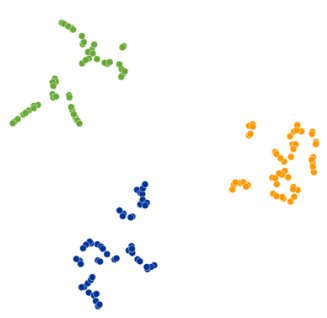
\includegraphics[scale=0.3]{abb/t-sne-example.png}
  \caption{Cluster Analyse angewendet auf 2-dimensionale Daten von 
    Wattenberg et al. \cite{wattenberg2016how}.
  }
\end{figure}

\subsubsection{Reinforcement Learning}
Bei diesem Paradigma liegen dem Lernalgorithmus zwar nicht die korrekten 
Output-Werte vor, aber der Lernalgorithmus erhält für jeden vorhergesagten Wert 
eine Rückmeldung, wie erwünscht dieser Wert ist. 
\[ 
  \mathbf{D} = (x_1, x_2, x_3, \dots, x_n) \subset X 
  \hspace{0.5cm}
  \text{und}
  \hspace{0.5cm}
  \texttt{score}: X \times Y \to \mathbb{R},
  \hspace{0.5cm}
  \texttt{score}(x_i, o_i) = s
\]
Wobei $x_i$ ein Input-Wert ist, $o_i$ der Output-Wert bei der 
Eingabe von $x_i$ ist und \texttt{score} eine Funktion die 
den Output $o_i$ bei gegeben $x_i$ bewertet.\\
Ein Beispiel ist ein Modell,
das mittels eines Lernalgorithmus darauf trainiert wird, ein Videospiel zu 
gewinnen. Der Lernalgorithmus bekommt ein Abbild von der Umgebung und gibt dem 
Spiel einen Input, welcher eine Aktion zufolge hat. Falls nun die Aktion dazu 
beiträgt, den Spieler in eine gute Position zu bringen oder gar das Spiel zu
gewinnen, bekommt die Aktion eine positive Bewertung, andernfalls eine
negative.\\\\
Die Problemstellung im maschinellen Lernen ist allgemein formuliert und abstrakt.
Dies ist der Grund, warum maschinelles Lernen in vielen unterschiedlichen 
Bereichen eingesetzt werden kann. Einer der Bereiche ist die natürliche
Sprachverarbeitung (engl. natural language processing), was uns zum nächsten 
Begriff führt. Natürliche Sprachverarbeitung wird im Folgenden 
mit NLP abgekürzt.
\pagebreak
\subsection{Semantische Vekorräume}
Das semantische Codieren von natürlicher Sprache in einem Vektorraum 
ist ein bedeutsames Problem in NLP
\cite{word2vec} ,\cite{reimers-2019-sentence-bert}.
Der resultierende Vektorraum kann
für verschiedene Problemstellungen (engl. downstream tasks) verwendet
werden. Ein Beispiel ist die Klassifizierung von Spam Nachrichten 
\cite{Ball2019}. Folgende Definitionen werden in dieser Arbeit 
für semantische Vektorräume verwendet.
\begin{definition}[Semantischer Vektorraum]
  \hfill\\
  Ein semantischer Vektorraum stellt Objekte als reelle Vektoren 
  dar, in einer Weise, dass ähnliche Objekte im projizierten 
  Vektorraum einen geringen Abstand zueinander haben.
\end{definition}
Hierfür ist es erforderlich vorher zu definieren, inwiefern zwei
Objekte ähnlich sind und welchen Abstandsbegriff man im Vektorraum 
wählt.
Der Begriff semantischer Vektorraum für natürliche Sprache heißt
hier, dass ähnliche Wörter, also Wörter mit ähnlicher Bedeutung 
im projizierten Vektorraum, einen geringen Abstand zueinander haben.  
In einem idealen semantischen Vektorraum würden
die Beziehung gelten, die in der Figur 2.3 dargestellt sind.
Wir werden die Vektoren im Folgenden als Embeddings bezeichnen.
\begin{figure}
  \begin{center}
      \begin{tikzpicture}
        \draw[thin,gray!40] (-3,-3) grid (3,3);
        \draw[->] (-3,-3)--(3,-3) node[right]{$x_1$};
        \draw[->] (-3,-3)--(-3,3) node[above]{$x_2$};
        \draw[line width=2pt,red,-stealth](-2,-2)--(1,-2) 
            node[midway, below]{weiblich};
        \draw[line width=2pt,red,-stealth](-1,1)--(2,1) 
          node[midway, above]{weiblich};
        \draw[line width=2pt,blue,-stealth](-2,-2)--(-1,1) 
            node[midway, left]{Geschichtsstudium};
        \draw[line width=2pt,blue,-stealth](1,-2)--(2,1) 
          node[midway, right]{Geschichtsstudium};
        \filldraw (-2,-2) circle (2pt)
        node[anchor=north east]{Mann};
        \filldraw (1,-2) circle (2pt)
        node[anchor=north west]{Frau};
        \filldraw (-1,1) circle (2pt)
        node[anchor=south east]{Taxifahrer};
        \filldraw (2,1) circle (2pt)
        node[anchor=south west]{Taxifahrerin};
    \end{tikzpicture}
  \end{center}
  \caption{Optimaler fiktiver semantischer Vektorraum}
\end{figure}
\subsubsection{Bag-of-Words}
Ein natürlicher Ansatz ist es, jedem Wort im vorliegenden Text eine Zahl 
zuzuordnen. Dadurch können sowohl die Häufigkeit eines Wortes als auch
die Sätze, in denen ein bestimmtes Wort vorkommt, effizient gefunden 
werden. Die Bedeutung eines Wortes ist hier komplett unabhängig von 
der Wahl der zugewiesenen Zahl. Das führt dazu, dass sogar Synonyme einen
hohen Abstand haben können.
\pagebreak
\begin{example}
  Sei $T = \{\text{Input}, \text{Mann}, \text{Frau},
   \text{Eingabe}\}$ eine Menge von Wörtern, dann ist die Zuordnung
  zu dem Vektorraum $\mathbb{N}^1$ wie folgt:
  \[
    \text{Input} \to 1, 
    \text{Mann} \to 2, 
    \text{Frau} \to 3,
    \text{Eingabe} \to 4.
  \]
  Obwohl Eingabe und Input semantisch sehr ähnlich sind, haben sie hier
  einen sehr unterschiedlichen Wert.
\end{example}
\begin{figure}
  \begin{center}
    \begin{tikzpicture}
    [inner sep=2mm,
     place/.style={circle,draw=blue!50,fill=blue!20,thick},
     transition/.style={rectangle,draw=black!50,fill=black!20,thick}]
    \node (i1) at (-3,4) {$1$};
    \node (i2) at (-3,2) {$0$};
    \node (dotsi1) at (-3,1) {$\vdots$};
    \node (i3) at (-3,0) {$0$};
    \node (L11) at (-1,4) [place] {$I_1$};
    \node (L12) at (-1,2) [place] {$I_2$};
    \node (dots1) at (-1,1) {$\vdots$};
    \node (L13) at (-1,0) [place] {$I_n$};

    \node (L21) at (2,4) [place] {$H_1$};
    \node (L22) at (2,2) [place] {$H_2$};
    \node (dots2) at (2,1) {$\vdots$};
    \node (L23) at (2,0) [place] {$H_n$};

    \node (L31) at (5,4) [place] {$O_1$};
    \node (L32) at (5,2) [place] {$O_2$};
    \node (dots3) at (5,1) {$\vdots$};
    \node (L33) at (5,0) [place] {$O_n$};

    \node (o1) at (7,4) {$0.1$};
    \node (o2) at (7,2) {$0.3$};
    \node (dotso1) at (7,1) {$\vdots$};
    \node (o3) at (7,0) {$0.8$};

    \draw[->] (i1) -- (L11);
    \draw[->] (i2) -- (L12);
    \draw[->] (i3) -- (L13);

    \draw[->] (L11) -- (L21);
    \draw[->] (L11) -- (L22);
    \draw[->] (L11) -- (L23);
    \draw[->] (L12) -- (L21);
    \draw[->] (L12) -- (L22);
    \draw[->] (L12) -- (L23);

    \draw[->] (L13) -- (L21);
    \draw[->] (L13) -- (L22);
    \draw[->] (L13) -- (L23);

    \draw[->] (L21) -- (L31);
    \draw[->] (L21) -- (L32);
    \draw[->] (L21) -- (L33);

    \draw[->] (L22) -- (L31);
    \draw[->] (L22) -- (L32);
    \draw[->] (L22) -- (L33);

    \draw[->] (L23) -- (L31);
    \draw[->] (L23) -- (L32);
    \draw[->] (L23) -- (L33);

    \draw[->] (L31) -- (o1);
    \draw[->] (L32) -- (o2);
    \draw[->] (L33) -- (o3);
    \end{tikzpicture}
    \caption{ Architektur des neuronalen Netzwerks von Word2Vec}
  \end{center}
\end{figure}
\subsubsection{Word2Vec}
Im Jahr 2013 veröffentlichten Mikolov et al.  
zwei Modellarchitekturen, mit der ein
neuronales Netzwerk effizient lernen kann, semantische Embeddings
zu produzieren
\cite{word2vec}.
Sie haben dazu auch eine Implementierung veröffentlicht die sie 
\textit{Word2Vec} \footnote{https://code.google.com/archive/p/word2vec/}
genannt haben.
In beiden Architekturen besteht das neuronale Netzwerk aus einem 
Hidden Layer, der nach dem Training die reellwertigen 
Vektorrepräsentationen enthält.
Der Aufbau bei beiden Modellen ist in Figur 2.4 dargestellt.
Es ist zu beachten, dass der Hidden Layer keine Aktivierungsfunktion 
besitzt, da er nur als lineare Transformation von einer 
One-Hot-Codierung zu einem reellwertigen Vektor dient.
One-Hot-Codierung produziert für jedes aus n Wörtern einen Vektor
$v \in \{0,1\}^n$. Dieser Vektor ist an einer Stelle mit einer Eins
und sonst überall mit einer Null versehen. Jede Position, an der eine
Eins ist, gibt es nur einmal und codiert so durch die Position ein Wort.
Der Output-Layer hat als Aktivierungsfunktion einen Softmax, der 
Softmax gibt Werte zwischen 0 und 1 zurück. Der Output ist also ein 
Vektor $v \in (0,1)^n$, daraus kann dann entweder je nach Anwendung 
durch One-Hot-Codierung ein oder mehrere Wörter abgeleitet werden.\\
Es gibt nun zwei unterschiedliche Strategien, das neuronale Netzwerk
zu trainieren. Die erste ist Skip-Gram, gegeben ein Wort, soll das
Modell die naheliegenden Wörter vorhersagen. Das heißt, es soll einem
Wort einen richtigen Kontext zuordnen. Das Modell wird dadurch die
Fähigkeit entwickeln, Wörter mit ähnlichen Kontexten ähnlichen 
Embeddings zuzuordnen.\\
Die zweite Methode ist Continous Bag-of-Words (CBOW),
bei der das Modell den Kontext eines Wortes erhält,
dass heißt es erhält die Wörter die links und rechts von dem Wort
sind als Input. Die Aufgabe besteht nun darin das Wort vorherzusagen
welches zum gegebenen Kontext passt.
Folglich soll das Wort, das zu dem gegebenen Kontext passt,
vorhergesagt werden.
Da ähnliche Wörter ähnliche Kontexte haben, neigt das Modell dazu,
ähnliche Outputs für ähnliche Kontexte zu lernen.\\
Die Word2Vec-Embeddings sind dann ähnlich, wenn ihre Kontexte,
in denen sie verwendet werden, ähnlich sind.  
Die Kontexte haben eine feste Größe, die am Anfang ausgewählt wird.
Wenn die Kontextgröße zu klein gewählt wird, kann es passieren, dass 
das Wort mit inhaltslosen Wörtern assoziiert wird, wie z.B. Artikel 
oder Präpositionen. Wenn die Kontextgröße zu groß ist, können 
unterschiedliche Kontexte verschwimmen und ungenaue Ergebnisse entstehen.
Folglich hat die Kontextgröße einen entscheidenden Einfluss auf den Erfolg 
des Modells. Vaswani et al. lösen das Kontextproblem 
durch die Transformer-Modellarchitektur \cite{transformer}.
\begin{figure}
  \begin{center}
    \begin{tikzpicture}
      [inner sep=2mm,
       place/.style={circle,draw=blue!50,fill=blue!20,thick},
       transition/.style={rectangle,draw=black!50,fill=black!20,thick}]
        \node (E) at (-2,0) [transition] {Encoder};
        \node (D) at (2,0) [transition] {Decoder};
        \node (I) at (-2,-2) {Input};
        \node (O) at (2,2) {Output};
        
        \draw[->] (I) -- (E);
        \draw[->] (E) -- (D);
        \draw[->] (D) -- (O);
        \draw[->] (O) -- (D);
      \end{tikzpicture}
  \end{center}
  \caption{Transformer-Architektur stark vereinfacht}
\end{figure}
\subsubsection{Transformer}
Die Transformer-Architektur \cite{transformer}
ist ein Meilenstein im NLP Bereich.
Die vorgestellte Deep Learning Architektur bildet die Basis
für BERT, \textit{SentenceTransformer} und Large Language-Models
(wie z.B. Chat-GPT).
Das Modell wurde ursprünglich entwickelt, um bei einem gegebenen
Satz 
einen sinnvollen neuen Satz zu generieren. Die Donwstream Task auf
die eine Implementierung der Architektur trainiert wurde,
ist das Übersetzen von Englisch zu Deutsch und von
Englisch zu Französisch. 
Der Transformer kann jedoch wieder zur Erzeugung semantischer Embeddings 
verwendet werden, wie im Abschnitt zum \textit{SentenceTransformer} erläutert
wird.
\begin{figure}
  \begin{center}
    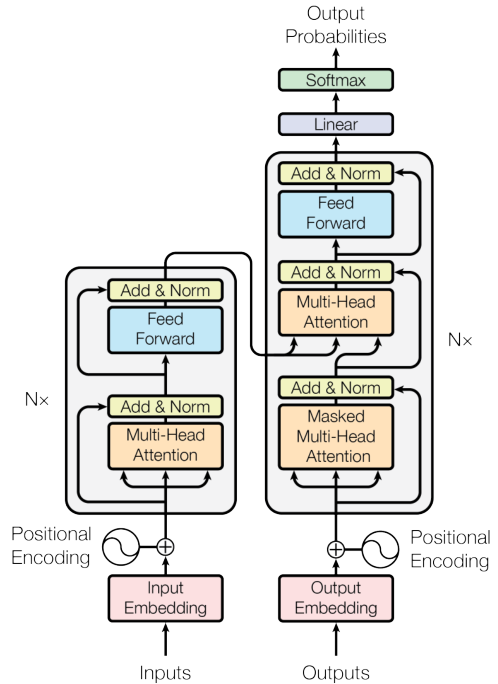
\includegraphics[scale=0.5]{abb/transformer-figure.png}
  \end{center}
  \caption{
      Die Transformer-Architektur entnommen aus der Veröffentlichung 
      von Vaswani et al. \cite{transformer}.
      Der linke Block ist der Encoder und der rechte Block der Decoder.
  }
\end{figure} 
Die Architektur hat zwei große Blöcke, die in der Abbildung 2.5
zusehen sind. Der erste Block ist der Encoder, dieser erhält die
Eingabe. Beim Übersetzen wäre das der zu übersetzende Text.
Der Encoder codiert den Input in semantische Embeddings und gibt
an, wie wichtig jedes Wort in dem Satz für ein anderes gegebenes
Wort ist.
Bei dieser Architektur gibt es keine Kontextgröße, sondern der
Kontext ist die gesamte Eingabe. Somit ist das Problem der 
Kontextgröße aus dem letzten Abschnitt gelöst.
Der Encoder bestimmt, welche Wörter wichtig sind und welche eher 
unwichtig sind in Bezug auf ein gegebenes Wort.
Der Decoder erhält den von ihm selbst produzierten Output sowie 
das Ergebnis des Encoders, um das nächste Wort zu generieren. 
Außerdem startet dieser mit einem konstanten Start-Embedding und 
um die Generierung zu stoppen, gibt er selbst ein konstantes 
Stopp-Embedding aus. Insbesondere ist es möglich, dass mehrere
Encoder und Decoder gleichzeitig hintereinander geschaltet werden 
können.\\
Die Architektur ist in Abbildung 2.6 dargestellt. Im Folgenden 
werden die wichtigsten Bestandteile der Abbildung erläutert.
{\bf Input-Embedding}
gibt dem Input, der in Textform vorliegt, eine Vektorrepräsentation.
Danach wird auf dem Vektor ein {\bf Positional Encoding} darauf
addiert.
Der Transformer verarbeitet alle Wörter parallel, deswegen geht die 
Positionsinformation verloren. Um diese Information trotzdem im 
Vektor 
zu codieren, wird für jede Position ein einzigartiger Vektor auf
das Wort-Embedding addiert. 
Im Block {\bf Add \& Norm} werden zwei Inputs addiert und dann 
normalisiert, damit die Werte in dem Modell nicht zu groß werden.
Feed Forward ist ein neuronales Netzwerk mit zwei Layern.
Alle Wort-Embeddings werden nacheinander und identisch in das
Netzwerk eingegeben. Der erste Input-Layer hat als 
Aktivierungsfunktion ein 
Softmax und der zweite hat die Identitätsfunktion.
Dann gilt für das Netzwerk:
\[
  FFN(x) =\text{max}(0, xW_1 + b_1)W_2 + b_2.
\]
Der {\bf Linear Block} ist wieder ein neuronales Netzwerk, mit allen
Aktivierungsfunktionen: $ f_{i,j}(x) = x $. 
Das {\bf Multi Head-Attention} Modul ist der wohl wichtigste 
Bestandteil der Architektur. Dieses gibt die Korrelation 
zwischen einem Wort und allen
Restlichen im Input aus. Der gesamte Input wird als Kontext 
betrachtet, aber das Modell lernt, auf welche Wörter es im 
Kontext viel oder wenig
Aufmerksamkeit schenken soll. Das {\bf Masked Multi Head-Attention}
Modul ist nur beim Trainieren anders als das Multi 
Head-Attention-Modul.
Beim Trainieren ist der Input des Decoders bereits der Satz,
den das Modell vorhersagen soll. Daher müssen alle Wörter, 
die es noch nicht vorhergesagt hat, verdeckt (engl. masked) werden.
\subsubsection{BERT}
Das BERT-Modell  
ist ein wichtiger Meilenstein im NLP-Bereich und kann 
als eines der ersten Large Language-Models betrachtet werden
\cite{conf/naacl/DevlinCLT19}.
Das Modell verbessert die Transformer-Architektur, 
indem es die Token-Embeddings verbessert, zwei neue Trainingsaufgaben einführt
und ausschließlich Encoder verwendet.
\begin{figure}
  \begin{center}
    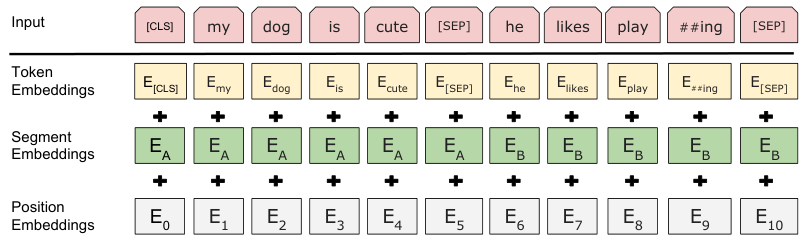
\includegraphics[scale=0.5]{abb/BERT-Tokens.png}
  \end{center}
  \caption{
    Der Token-Embedding-Prozess entnommen aus der Veröffentlichung
    von Devlin et al.
    \cite{conf/naacl/DevlinCLT19}.
  }
\end{figure}
In Abbildung 2.7 ist der Token-Embedding-Prozess abgebildet,
der im Folgenden näher beschrieben wird. Zunächst ist es 
notwendig zu erläutern, was ein Token ist. Ein Token ist in 
diesem Fall ein Wort, 
aber generell die kleinste bedeutungstragende Einheit im
Sprachsystem. Die Aufteilung eines Textes in Tokens vereinfacht
die weitere Verarbeitung.\\
Das BERT Modell kombiniert drei unterschiedliche Informationen
in Vektorform, um noch bessere Token-Embeddings als die 
Token-Embeddings von dem Transformer zu generieren. BERT
verwendet \textit{WordPiece} 
\cite{wu2016googlesneuralmachinetranslation},
um die rohen Tokens in Vektoren umzuwandeln.
Auf diese werden nun ein Segment-Embedding und schließlich die
Position-Embeddings addiert.
Das {\bf Segment-Embedding} codiert die Information,
welche Tokens zu welchen Satz gehören.
Das {\bf Position-Embedding} codiert die globale sequenzielle
Position im Input.\\
Die beiden unterschiedlichen Trainingsaufgaben stellen das wichtigste
Puzzleteil dar. Während der Transformer die Tokens von links nach rechts
vorhersagt, wird BERT darauf trainiert, Wörter vorherzusagen, die auf
beliebiger Position fehlen. Dadurch erhält das Modell Zugang zu dem
Kontext, der sich links und rechts von dem zu prädizierenden Token befindet.
Diese Trainingsform wurde {\bf Masked Language-Modeling} von 
Wu et al. benannt.
Bei diesem Verfahren werden $15 \%$ der Input-Token entweder durch das
\verb|[Mask]| Token oder durch einen zufälligen anderen Token ersetzt.
Dabei bleiben $10 \%$ der Token, die maskiert werden sollten,
unverändert. Weitere $10 \%$ der Token, die maskiert werden sollten,
werden durch ein zufälliges anderes Token ersetzt, während die
restlichen $80 \%$ durch das \verb|[Mask]| Token ersetzt werden.\\
Die zweite Trainingsaufgabe ist {\bf Next Sentence-Prediction} (NSP),
bei dieser Aufgabe soll das BERT Modell bei der Eingabe von zwei Sätzen 
entscheiden, ob diese sequenziell nacheinander kommen oder nicht.
Bei der einen Hälfte der Daten handelt es sich um zwei Sätze, die nacheinander 
auftreten. Bei der anderen Hälfte der Daten handelt es sich um zufällige,
nicht sequenzielle Sätze. Zur Inferenz des Modells, ob die Sätze
nacheinander kommen oder nicht, wird ein Token \verb|[cls]| 
eingeführt, welches beim Input immer an erster Stelle steht.
Der erste Output-Vektor des BERT-Modells ist das Ergebnis des
\verb|[cls]| Tokens und wird verwendet, um den Output
\verb|isNext| oder \verb|notNext| zu produzieren.\\
Nach dem Training erhält man aus dem BERT-Modell für jeden 
Input-Vektor genau einen Output-Vektor. 
\subsubsection{Sentence Transformer}
Das Sentence-BERT-Modell \cite{reimers-2019-sentence-bert}
ist der aktuelle Stand der Technik im semantischen Codieren 
von natürlicher Sprache in einem Vektorraum. Die Implementierung 
ist unter dem Namen \textit{SentenceTransformer} 
\footnote{https://sbert.net} von Reimers et al. bekannt.
Die Motivation hinter Sentence-BERT (SBERT) ist das effiziente
semantische Vergleichen 
von zwei Sätzen. Wenn man mit BERT herausfinden möchte, wie semantisch
ähnlich zwei gegebene Sätze sind, dann ist es erforderlich, dass beide
Sätze als Input in das Modell eingeben. Das heißt, wenn die Ähnlichkeit 
von allen $n$ Sätzen jeweils zueinander herausgefunden werden soll,
gibt es $\frac{n(n-1)}{2}$ Eingaben in das BERT Modell.
Bei SBERT kann dagegen jeder Satz einzeln eingegeben werden und der
resultierende Output ist dann ein semantischer Vektor. Um die
semantische Ähnlichkeit zwischen zwei Vektoren zu erhalten,
müssen beide Vektoren lediglich in eine zu wählende Metrik
eingesetzt werden. 
%wird die Kosinus-Ähnilichkeit verwendet: Sei $u,v \in \mathbb{R}^n$, dann setze
%\[
%  Kos(u,v) := cos(\phi) = \frac{u \cdot v}{\|u\|\|v\|} 
%  = \frac
%  {
%    \sum_{i=1}^n u_iv_i
%  }
%  {
%    \sqrt{\sum_{i=1}^n u_i^2} \sqrt{\sum_{i=1}^n v_i^2}
%  }.
%\]
Dies ermöglicht es, die semantische Ähnlichkeit zwischen zwei Vektoren 
effizient zu berechnen.\\
Die Modellarchitektur von SBERT wird als {\bf Siamese Neural Network }
bezeichnet, da zwei unterschiedliche BERT-Modelle verwendet werden,
um beide Sätze in einen Vektor umzuwandeln, aber beide Modelle
teilen sich die Gewichte. In der Abbildung 2.8 ist die Siamese 
Neural Network zusehen.\\
\begin{figure}
  \begin{center}
    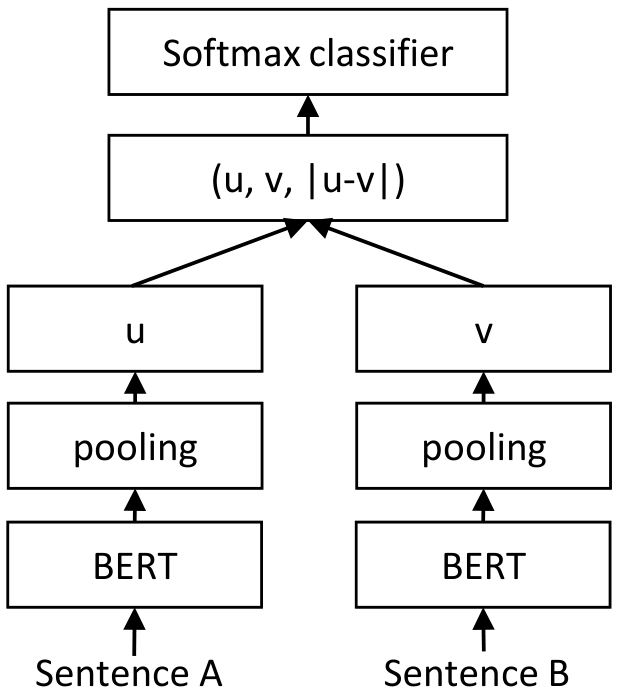
\includegraphics[scale=0.3]{abb/SBERT.png}
  \end{center}
  \caption{
    Die SBERT-Architektur entnommen aus der Veröffentlichung
    von Reimers et al.
    \cite{reimers-2019-sentence-bert}. 
    Beide BERT-Modelle teilen sich dieselben Gewichte. 
  }
\end{figure}
Die Output-Vektoren von den zwei BERT-Modellen werden schließlich 
in ein Pooling-Modul eingeben. 
{\bf Pooling} ist das zusammenfassen von vielen Vektoren 
in eine geringere Anzahl von Vektoren oder Dimensionen. In diesem 
Fall werden die $n$ Output-Vektoren von den zwei BERT-Modellen in
einen einzigen Output-Vektor transformiert. Das Default Pooling
von dem \textit{SentenceTransfomer} ist der Mittelwert, d.h.
auf alle  Einträge der Output-Vektoren von den BERT-Modellen
wird das arithmetische Mittel angewendet.
Daraus erhält man einen Vektor mit den jeweiligen gemittelten 
BERT-Output-Vektoren.\\
Das BERT Modell wird  vorher an die spezielle Aufgabe 
angepasst, zwei Vektoren semantisch zu vergleichen. 
Dafür wird der SNLI Datensatz verwendet, dieser beinhaltet immer 
zwei Sätze mit drei möglichen Labels: 
\verb|contradiction|, \verb|neutral|, und \verb|entailment|.
SBERT soll für zwei Sätze vorhersagen, ob sie sich inhaltlich
widersprechen, neutral zueinander sind oder ob der eine Satz
eine Fortsetzung des anderen ist. Daraus lernt das Modell,
ein semantisches Verständnis für Sätze zu erlangen.\\
Beim Training wird zur Ermittlung der Label-Vorhersage ein 
neuer Output-Vektor kreiert, indem die beiden 
Pooling-Output-Vektoren und ihre Differenz miteinander 
konkateniert werden.
Anschließend wird dieser neue Output-Vektor mit einer Matrix,
welche durch das Training erlernte Gewichte enthält, multipliziert, 
sodass ein Vektor mit drei Dimensionen entsteht.
Danach wird der Softmax auf alle Einträge des finalen 
Output-Vektors angewendet. Die Position in dem Vektor mit dem 
höchsten Wert wird schließlich dem zugehörigen Label zugeordnet.
Mathematisch:
Sei $W \in \mathbb{R}^{3 \times (2\cdot n + 1)}$ die Matrix,
die die Gewichte enthält, 
$u,v \in \mathbb{R}^n$ die Output-Vektoren von dem Pooling-Modul,
$\texttt{concat}$ die Funktion die drei Vektoren konkateniert und
$|\cdot|$ eine beliebige Norm, dann
\[
  o_i = \text{softmax}((W \cdot \texttt{concat}(u,v, |u-v|))_i), \text{ für } i = 1, 2, 3.
\]
Nachdem Training bei der Inferenz wird der Vektor, nachdem 
Pooling-Modul als Output-Vektor ausgeben. SBERT liefert 
also ein Tool, um Sätze semantisch in einem Vektorraum abzubilden,
welches sich in späteren Kapiteln als sehr hilfreich herausstellt.
\subsection{Code Llama}
Die \textit{Code-Llama}-Familie an Large Language-Models wurde von 
Rozière et al. im Jahre 2024 entwickelt
\cite{rozière2024codellamaopenfoundation}.
{\bf Large Language-Models} sind Modelle, die auf
einer großen Menge von Daten trainiert wurden, welche sich darin
auszeichnen, natürliche Sprache verstehen sowie generieren zu
können und deswegen in der Lage sind, eine Vielzahl von Aufgaben
im NLP-Bereich zu lösen.\\
Code Llama ist das auf Programmiersprachen 
spezifische Aufgaben optimierte vorangegangene Llama-2-Modell.
Das LLama-2-Model wird,
um zum resultierenden Code Llama zu kommen, erneut auf einem neuen
Datensatz trainiert. Dieser besteht aus drei verschiedenen 
Kategorien von Daten. Der größte Teil im Datensatz,
mit $85 \%$ wurde zufällig aus einen $859$ GB großen Datensatz,
aus Programmiersprachen spezifischen Aufgaben entnommen,
indem das Modell darauf trainiert wird, fehlende Programmzeilen in 
einer vergebenen Lücke zu füllen. Dabei kann es sich um Programmcode,
aber auch um Kommentare handeln. Der zweitgrößte Teil im Datensatz,
mit $8 \%$ wurde zufällig aus einen $78$ GB großen Datensatz entnommen,
welcher aus natürlicher Sprache besteht, in der es um 
Programmcode geht. Dieser Teil beinhaltet Diskussion über Quellcode
sowie Fragen und Antworten, welche sich auf Quellcode beziehen. 
Der kleinste Teil im Datensatz mit $7 \%$ wurde zufällig aus einen 
$3.5$ TB großen Datensatz entnommen und
besteht aus beliebiger natürlicher Sprache, damit das Modell
seine alten Fähigkeiten erhält.\\
Das LLama-2-Modell ist eine Verbesserung des Llama-Modells.
Dieses wurde auf neueren Daten trainiert und verwendet 
$40 \%$ mehr Tokens, die Llama-Famillie besitzt je nach Modell
$1.0-1.4$ Billionen Tokens und die gesamte Llama-2-Famillie 
besitzt $2.0$ Billionen.
Außerdem wurde die Kontextlänge verdoppelt und
es gab eine Veränderung in der Llama-Transformer-Architektur. 
In den Attention-Modulen werden zwei Werte, die normalerweise 
immer wieder berechnet werden, geteilt, was bedeutet, dass 
jedes Attention-Modul Zugriff auf die gleichen Werte hat.
Dies führt zu geringfügig schlechteren Ergebnissen, jedoch zu
einer deutlichen Leistungssteigerung.\\
Das Llama-Modell wiederum besteht aus einer Decoder-only-Transformer-Architektur.
Der {\bf Decoder-only-Transformer}
besteht lediglich aus Decoder-Transformer-Blöcken,
wie der Name bereits vermuten lässt. Bei dieser Architektur
ist der anfängliche Input des Decoders die Eingabe des Nutzers.
Auf diese Eingabe wird dann immer wieder das neu generierte Token
drauf konkateniert. Auf diese Weise wird die Eingabe nicht explizit
von dem bereits generierten getrennt, sondern beides wird als 
gleicher Kontext verwendet.\\
Das Besondere an Llama ist, dass es nur auf frei verfügbaren
Daten trainiert wurde und dass das Modell Open Source ist. Der
Datensatz besteht aus English Common Crawl [$67\%$],
C4 [$15\%$],  Github [$4.5\%$],
Wikipedia [$4.5\%$], Gutenberg and Books3 [$4.5\%$], 
ArXiv [$2.5\%$], und Stack-Exchange [$2\%$].\\
Code Llama ist eine Open Source-Software, die unter allen 
verfügbaren Modellen am besten in multilingualen Benchmarks 
abschneidet. Multilingual bedeutet die Verwendung mehrerer 
Programmiersprachen. Diese Eigenschaften machen es sehr geeignet
für diese Arbeit.
\subsection{Code2Vec}
 \textit{Code2Vec}  ist eine im Jahre 2018 von Alon et al. 
entwickelte Modellarchitektur, die Quellcode in einen semantischen 
Vektor kodiert
\cite{code2vec}.
Nach den Erfolgen in NLP, natürliche Sprache 
in semantische Vektoren zu kodieren, entstand der Wunsch, auch 
Quellcode in semantischen Vektoren abzubilden. Mit diesen Vektoren 
können dann wieder viele verschiedene Aufgaben gelöst werden.
Das motivierende Beispiel bei \textit{Code2Vec} ist die Vorhersage 
eines sinnvollen Namens für eine Funktion. Die Architektur, welche 
in Abbildung 2.9 dargestellt ist, wird im Folgenden erläutert. 
\begin{figure}
  \begin{center}
    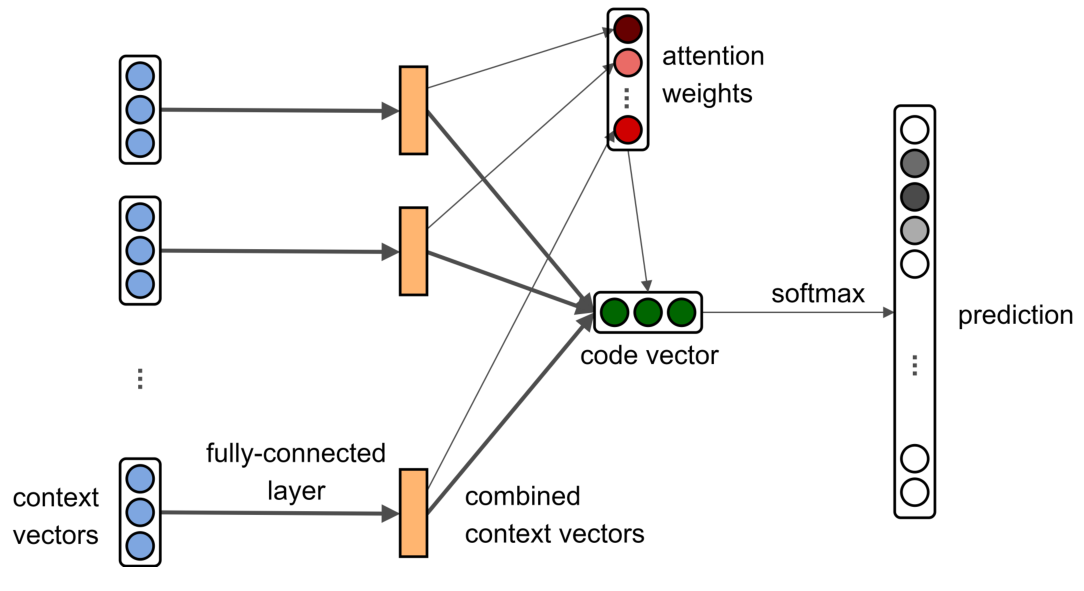
\includegraphics[scale=0.3]{abb/code2vec.png}
  \end{center}
  \caption{
    Die \textit{Code2Vec}-Architektur entnommen aus der 
    Veröffentlichung von Alon et al.
    \cite{code2vec}
  }
\end{figure}
Alon et al. fanden heraus, dass eine geeignete Darstellung
von Quellcode als ein mathematisches Objekt ein abstrakter 
Syntaxbaum ist. Dieser erhält die strukturellen Zusammenhänge
zwischen den Tokens und kann gut in einen Vektor codiert werden.
Die Input-Vektoren (Context-Vectors) bestehen jeweils aus einem
Pfad im abstrakten Syntaxbaum, mit dem jeweiligen Starttoken und
Endtoken des Pfades. Danach folgt ein Hidden Layer, mit \texttt{tanh}
als Aktivierungsfunktion. Der endgültige Vektor wird als lineare 
Kombination aus den Output-Vektoren und den Attention-Weights 
berechnet. Sei $h_1, \dots, h_n \in \mathbb{R}^d$ die Output-Vektoren 
von dem Hidden Layer
und $\alpha \in \mathbb{R}^n$ der Attention-Weights Vektor.
\[
  \verb| code vector | v = \sum_{i = 1}^n \alpha_i \cdot h_i
\]
\\
\pagebreak
\hfill\\
Mit dem \verb|Code-Vector| kann dann das gewünschte Label vorhergesagt 
werden. Das Modell kann demnach darauf trainiert werden, bei gegebenem 
\verb|Code-Vector| bzw. Quellcodeauszug ein bestimmtes Label in 
natürlicher Sprache vorherzusagen. Nachdem das Training abgeschlossen 
ist, kann es ein Label für einen Quellcode vorhersagen, welches nicht 
im Trainingssatz enthalten ist. 
Die Trainingsart ist demnach überwachtes Lernen, was eine Aufbereitung der
Daten benötigt. Das Modell kann lediglich die Labels vorhersagen, die es 
vorher im Training gesehen hat.
\subsection{ T-Distributed Stochastic Nieigbor Embedding}
{\bf T}-Distributed {\bf S}tochastic {\bf N}eigbor {\bf E}mbedding
({\bf  t-SNE}) ist ein Algorithmus, welcher zum Visualisieren von
hochdimensionalen Daten eingesetzt wird
\cite{JMLR:v9:vandermaaten08a}. Um das zu ermöglichen,
reduziert  \textit{t-SNE} die Dimension von $n \in \mathbb{N}$ zu
einer niedrigeren Dimension wie zwei oder drei, in der der 
Mensch die Datenpunkte leicht interpretieren kann. Dabei versucht
der Algorithmus, die Nachbarschaftsverhältnisse der Datenpunkte
möglichst zu erhalten.\\
Im Folgenden wird der Algorithmus skizziert und danach wird aufgezeigt,
was bei der effektiven Verwendung von \textit{t-SNE} zu beachten ist. Die
hochdimensionalen Datenpunkte werden mit $\mathbf{H}$ und die 
niedrigdimensionalen Datenpunkte mit $\mathbf{N}$ bezeichnet. Der erste Schritt 
des Algorithmus ist es, jedem Datenpunktpaar im Datensatz $\mathbf{H}$
einen Ähnlichkeit-Score zuzuweisen. Dieser wird berechnet, indem man 
zuerst die euklidische Distanz von jedem Datenpaar berechnet und dann das 
Ergebnis in eine Wahrscheinlichkeitsverteilung eingibt. Dies führt zu
einer Normalisierung des Wertes. Das Ergebnis ist dann eine Tabelle mit 
einem Ähnlichkeit-Score für jedes Datenpaar in $\mathbf{H}$.\\
Als Nächstes werden die Datenpunkte zufällig in der niedrigen Dimension 
$\mathbf{N}$ angeordnet. Die nachfolgenden zwei Schritte werden 
$T\in \mathbb{N}$ 
mal wiederholt, wobei $T$ ein Parameter ist, der wählbar ist.
\begin{enumerate}
  \item Berechne Ähnlichkeit-Score von $\mathbf{N}$, diesmal wird aber die
      studentische t-Verteilung als wahrscheinlichkeitsverteilung genommen. 
  \item Verschiebe die Datenpunkte von $\mathbf{N}$ um ein kleinen Wert in
    die Richtung, die den Unterschied der Ähnlichkeit-Score von $\mathbf{H}$
    und $\mathbf{N}$ minimiert.
\end{enumerate}
Nach $T$ Wiederholung ist der Ähnlichkeit-Score von $\mathbf{N}$ und 
$\mathbf{H}$ nahe bei einander, d.h. die Nachbarschaftsverhältnisse 
von $\mathbf{N}$ und $\mathbf{H}$ sind nun ähnlich.\\
Wattenberg et al. haben untersucht, wie man  \textit{t-SNE} sinnvoll
anwendet und welche Schlüsse man aus der Visualisierung 
ziehen kann \cite{wattenberg2016how}. 
Sie fanden heraus, dass die Wahl der Parameter 
für das Ergebnis eine wichtige Rolle spielen. Die wichtigsten 
Parameter sind die Iterationen $T\in \mathbb{N}$ und die Perplexity 
$P \in \mathbb{N}$.\\
Eine geeignete Iteration $T$ kann relative einfach durch ausprobieren 
herausgefunden werden: Falls sich die Datenwolke bei Erhöhung
von $T$ nicht mehr wirklich verändert, ist die Anzahl der Iteration
$T$ gefunden. 
\pagebreak
\hfill\\
Die Perplexity kann intuitiv als Schätzung für die Anzahl an nahen 
Nachbarn, die jeder Datenpunkt hat, gesehen werden.
Die Suche nach einer geeigneten Perplexity ist schwieriger, 
da wir die Anzahl der Nachbarn in den hochdimensionalen 
Daten häufig nicht kennen. Van der Maaten et al., welche  
\textit{t-SNE} entwickelt haben,
empfehlen eine Perplexity $P \in \{5,6, \dots, 50\}$ 
\cite{JMLR:v9:vandermaaten08a}.
Außerhalb dieses Bereichs kann es zu unerwünschten Ereignissen 
kommen. Bei $P=2$ haben Wattenberg et al. herausgefunden, 
dass  \textit{t-SNE} bei einer zufällig generierten Datenwolke 
fälschlicherweise kleine Gruppierungen (engl. cluster) bildet. 
Falls $P$ größer ist als die Anzahl der Datenpunkte, ist das
Ergebnis überhaupt nicht interpretierbar. Es ist daher ratsam,
mehrere Werte für $P$ zu verwenden, um sicherzustellen, 
dass  \textit{t-SNE} keine falschen Nachbarschaftsbeziehungen darstellt.\\
Wattenberg et al. stellten außerdem fest, dass sowohl die 
Information des Durchmessers eines Clusters als auch die Abstände 
zwischen einem Cluster und einem anderen durch  \textit{t-SNE}
vollständig  verloren gehen. Nach Betrachtung der  
\textit{t-SNE} Ausgabe kann daher 
keine Aussage über den Durchmesser eines Clusters, die Position 
des Clusters und die Lagebeziehungen zwischen Clustern getroffen 
werden.\\
Der  \textit{t-SNE} Algorithmus ist ein wichtiges Tool, um qualitative
Aussagen über Daten zu treffen. Es ist jedoch wichtig, mehrere 
Parameter auszuprobieren. Es kann nur eine Aussage über die 
Existenz von Clustern gemacht werden, nicht über ihre geometrischen 
Gegebenheiten. Wenn diese Bedingungen beachtet werden, kann  \textit{t-SNE}
ein mächtiges Visualisierungs-Tool sein, um eine Intuition für die
Anordnung der Datenpunkte zu erlangen.

% effective use paper: 
% https://distill.pub/2016/misread-tsne/?_ga=2.135835192.888864733.1531353600-1779571267.1531353600
%pgf plots

%\subsection{Stand der Technik} in Introduction
% Self supervised learning (JTrans, PalmTree)
% Same Source policy (Safe)
%  Clap
\pagebreak
\section{Methodik}
\subsection{Datensatz}
Im maschinellen Lernen hat der Datensatz bzw. die Trainingsdaten
den größten Einfluss auf die Güte des Modells. Wir haben uns 
für die Open Source-Standard-C-Bibliothek von GNU entschieden. 
Die Sprache C wurde gewählt, da sie die zweitpopulärste Sprache 
nach C++ ist, die zu Maschinencode kompilierbar ist.
\footnote{\url{https://www.jetbrains.com/lp/devecosystem-2024/}}
Die GNU-Bibliothek wurde aufgrund der hohen Qualität des 
Quellcodes ausgewählt, da das Projekt seit 1987 existiert 
und die Community jederzeit auf Fehler im Quellcode hinweisen kann.
Zum anderen wird die Bibliothek weitgehend in vielen Applikationen 
eingesetzt.\\
Der wichtigste Aspekt ist, dass man mit diesem Datensatz 
die Ergebnisse des trainierten Modells vergleichen kann, da die 
C-Bibliothek im POSIX-Standard festgelegt ist und mehrfach 
implementiert wurde. Dadurch erhält man mehrere hochqualitative 
Quellcodeprojekte, die die gleiche Semantik aufweisen. Die 
unterschiedlichen Implementierungen werden zu unterschiedlichem 
Assemblercode kompiliert. Deswegen kann mit unterschiedlichen 
Standard-C-Bibliotheken, die den POSIX-Standard implementieren,
getestet werden, ob das finale Modell beide Implementierungen 
als sehr ähnlich klassifiziert.

% Warum ist die Auswahl des Datensatzes wichtig
% Warum Glibc? 
% Gleicher Standard mit gleicher Semantik unterschiedlich Implementierung
\subsection{Datenpipeline}
Der große praktische Teil der Arbeit bestand darin, eine große 
Menge an Daten in unterschiedliche Darstellungen umzuwandeln. 
Jeder Zwischenschritt wurde gespeichert, um nicht jede Darstellung 
erneut generieren zu müssen. Im Folgenden wird die generelle Architektur,
wie Daten verarbeitet werden (engl. pipeline), vorgestellt, um einen 
Überblick über den praktischen Teil dieser Arbeit zu geben.
\begin{figure}
  \begin{center}
    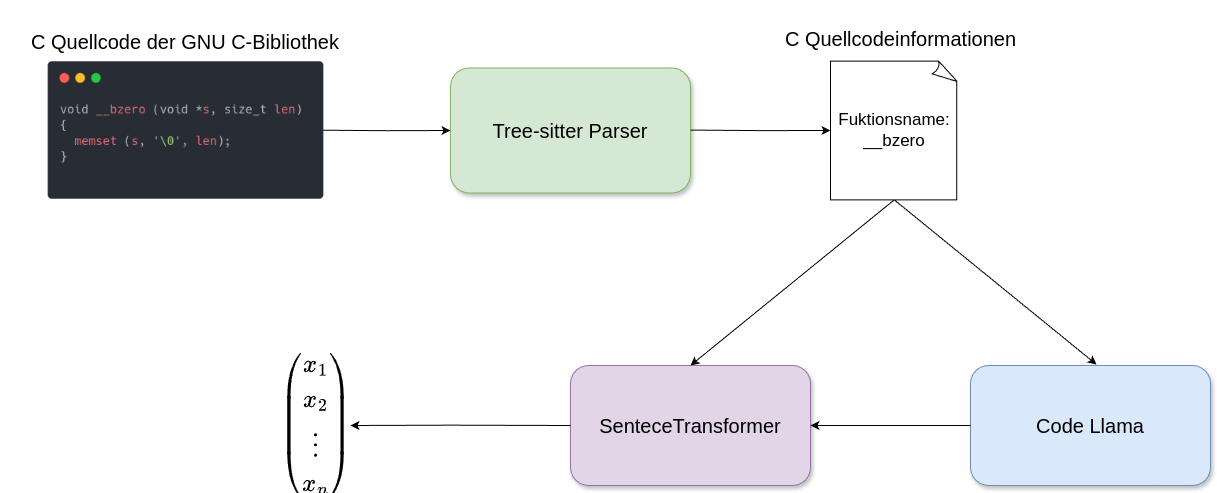
\includegraphics[scale=0.35]{abb/data-pipeline-2.drawio.png}
  \end{center}
  \caption{
    Die Datenpipeline dargestellt, dabei 
    sind Vierecke mit abgerundeten Ecken Tools, die Daten in eine 
    andere Darstellung umwandeln.
  }
\end{figure}\\
Die Rohdaten entsprechen dem unverarbeiteten 
C-Quellcode aus der GNU-Standard-C-Bibliothek. 
Wir benötigen nicht alle Teile des Quellcodes, sondern nur bestimmte.
Wir betrachten ausschließlich nur Funktionen, d.h. wir wollen
bspw. alle Datenstrukturen, die in dem Quellcode definiert werden,
aus dem Quellcode entfernen. Die Zerlegung und Umwandlung des
Inputs in sinnvolle Teile wird Parsing genannt.\\
In dieser Arbeit wurde {\bf Tree-sitter} 
\footnote{\url{https://tree-sitter.github.io/tree-sitter/}} als
Parser verwendet, welcher
alle populären Programmiersprachen in Syntaxbäume umwandeln kann.
Ursprünglich wurde \textit{Tree-sitter} für den Texteditor Atom
entwickelt und wird heute noch in vielen Texteditoren bspw. 
für die Hervorhebung von Syntax verwendet. Generell kann 
\textit{Tree-sitter} jedoch
für alle Anwendungen benutzt werden, die Informationen aus Quellcode
verarbeiten wollen. Aus dem von \textit{Tree-sitter} generierten
Syntaxbaum kann dann jegliche gewünschte Information entnommen 
werden.\\
Die Quellinformationen werden immer zunächst gespeichert, damit die 
Verarbeitung beim nächsten Mal an diesem Punkt beginnen kann.
Die Quellinformationen beziehen sich immer auf eine Funktion,
deswegen bestehen die Daten aus einem Tupel, der aus je einer
Funktion und den gewünschten Quellinformationen besteht.\\
Nachdem die Quellcode-Informationen extrahiert wurden, 
gibt es eine Abzweigung in der Datenpipeline, entweder 
werden die Quellinformationen von Code Llama nochmal in natürlicher 
Sprache beschrieben und dann in den \textit{SentenceTransformer}
eingegeben oder die Quellinformation wird direkt in den 
\textit{SentenceTransformer} eingegeben. Schließlich erhält man
wieder eine Datenmenge, die aus Tupeln besteht. Ein Tupel besteht
aus dem Funktionsnamen und dem zugewiesenen Embedding. 
Bei dieser Architektur kann mühelos jedes Tool ausgewechselt werden,
solange die Ausgabeformate eingehalten werden. 
% Treesitter erklären
% Source Code information in json datei speichern
% Dann Source code information in Vektor umwandeln
% Modularität -> Vorteile dieses Designs 
\subsection{Stabilität von SentenceTransformer}
Im vorherigen Abschnitt haben wir festgestellt, dass der endgültige
Schritt für alle Daten der \textit{SentenceTransformer} ist, deshalb
bildet 
er das Herzstück der Datenpipeline. In dieser Arbeit sollen 
verschiedene Beschreibungen des Quellcodes in 
natürlicher Sprache verglichen werden. Es ist wichtig, dass alle 
anderen Elemente in der Datenpipeline konstante Ergebnisse 
liefern und nicht schwanken. Aus diesem Grund wird im Folgenden 
untersucht, wie sich der \textit{SentenceTransformer} bei selber
Eingaben verhält. Im Optimalfall sollte der SentenceTransfomer bei 
selbem Input dasselbe Ergebnis liefern.\\
Um dies zu überprüfen, wurden $n = 100$ 
Code-Llama-Quellcode-Erklärungen zufällig ausgewählt und 
anschließend in
den SentenceTransformer $m = 100$ Mal eingegeben. Dabei beträgt
der höchste Abstand von zwei Vektoren,
die aus der gleichen Erklärung resultiert sind 
$d = 6.661338\cdot 10^{-16}$. Der 
Abstand ist ausreichend klein, um ihn in der Evaluation zu 
vernachlässigen. Der \textit{SentenceTransformer} ist daher
für die Anwendung in dieser Arbeit ausreichend stabil.

% Label Prozess sollte stabil sein bzw. deterministisch, sonst
% kann keine aussage über die Güte der Labels getätig werden
% Tabelle mit Ergebnissen der standardabweichungen
%
\pagebreak

\begin{figure}
  \begin{center}
    \begin{minipage}[c]{6cm}
        \centering
        \inputminted[fontsize=\scriptsize]{c}{comments.c}
    \end{minipage}
    \hspace{0.1cm}
    \begin{minipage}[c]{6cm}
        \centering
        \inputminted[fontsize=\scriptsize]{json}{comments.json}
    \end{minipage}
  \end{center}
  \caption{Links ein Quellcode-Beispiel und rechts der extrahierte Kommentar}
\end{figure}

\subsection{Funktionskommentare}
Bevor ein Programm kompiliert wurde, gibt es eine Menge an
Informationen, die den Inhalt der Funktion in natürlicher Sprache 
beschreiben. Eine offensichtliche Quellcode-Information, die im
Optimalfall den Inhalt der Funktion in natürlicher Sprache 
beschreibt, ist der Kommentar. Ein gelungener Kommentar zu einer
Funktion beschreibt die Kernfunktion der Prozedur, d.h. den Input,
den Output und die Umwandlung. Dieser Kommentar kann dann in den 
\textit{SentenceTransformer} eingeben werden und so in einen
Vektorraum abgebildet werden.\\
% Warum könnten funktionskommentare dafür geignet sein die Semantik einer
% Funktion zu beschreiben
Das Parsen der Kommentare wurden mit \textit{Tree-sitter} realisiert,
wie im Abschnitt zur Datenpipeline erwähnt. Dabei gab es eine große
Designentscheidung zu treffen, welche Kommentare in einer Funktion
berücksichtigt werden sollen.
Im Rahmen dieser Arbeit werden ausschließlich Kommentare verwendet,
die direkt  über der Funktion in stehen. Diese Designentscheidung
wurde unter der Hypothese getroffen, dass die einzeiligen
Kommentare innerhalb der Funktion meistens kein großen
Informationsgehalt haben, sondern auf
Gefahren oder Designentscheidungen hinweisen.
%(Beleg maybe: A survey on Reasearh of code comment). 
Hierbei sollte man aufpassen, dass der Prozess des Parsen nicht zu
speziell an die vorliegenden Datensatz angepasst wird, sonst 
verliert er seine Allgemeingültigkeit. 
% Probleme beim Parsen, wo sucht man nach Kommentaren?
% Keine einheitliche Konvention
% -> Unterschiedliche Code Base Unterschiedliche Kommentar Konventionen
\subsection{Code2Vec}
Das Besondere an \textit{Code2Vec} ist, dass der Quellcode in einem
abstrakten Syntaxbaum kodiert wird. Dies ermöglicht die Verwendung aller
Quellcode-Informationen, die im Quellcode enthalten sind. Anschließend wird
das Modell darauf trainiert, eine Eigenschaft in natürlicher Sprache
über den Quellcode vorherzusagen.\\
Bei dieser Herangehensweise, Vektoren zu erzeugen, wird
also kein \textit{SentenceTransformer}
verwendet, sondern die Vektoren werden durch Training des
\textit{Code2Vec} Modells als Nebenprodukt erzeugt. 
Das Modell wird hier, wie in der Implementierung von 
Alon et al., darauf trainiert Funktionsnamen vorherzusagen
\cite{code2vec}.
Die Implementierung des \textit{Code2Vec} Modells
nutzte Java als Datensatz, weshalb einige Anpassungen notwendig waren,
um das Modell auf C-Quellcode zu trainieren.\\
Das \textit{Code2Vec}-Modell basiert auf überwachtem Lernen,
deswegen wird der Datensatz vor dem Training zunächst aus
dem rohen Quellcode aufbereitet.\\
% Warum könnte \textit{Code2Vec} semantisch gute Vektoren produzieren
Um das \textit{Cod2Vec}-Modell zu trainieren,
ist es notwendig,
aus dem rohen Quellcode einer Funktion jeweils einen abstrakten 
Syntaxbaum und den
Funktionsnamen zu extrahieren. Alon et al. stellen ein Tool 
für Java zur Verfügung, welches das Extrahieren von abstrakten 
Syntaxbäumen und Funktionsnamen aus Java-Quellcode ermöglicht, 
deswegen war hier ein externes Tool notwendig.\\
Mit dem ASTminer von Kovalenko et al. können abstrakte Syntaxbäume
und Funktionsnamen extrahiert werden \cite{kovalenko2019pathminer}. 
Das Tool wurde vom JetBrains-Research-Team entwickelt, um Quellcode
in abstrakte Syntaxbäume (AST) zu 
kodieren, die als Input-Format für maschinelles Lernen dienen.\\ 
Für die Implementierung des \textit{Code2Vec}-Modells ist es 
erforderlich, dass der Datensatz ein bestimmtes Format aufweist.
Ein Trainingsbeispiel besteht jeweils aus einem 
Funktionsnamen, dem Label und einer Liste von Kontexten, welche den AST 
repräsentieren. Ein Kontext besteht aus einem Starttoken, einem Endtoken 
und einer Pfadbeschreibung vom Starttoken bis zum Endtoken.\\
Dieses \textit{Code2Vec}-Format kann durch eine zusätzliche Option
in der Konfiguration des \textit{ASTminers} generiert werden.
Obwohl diese Option mit "code2vec" betitelt ist, ist der Output des
\textit{ASTminers} nicht direkt von \textit{Code2Vec} verwendbar.
Das Tool weist nämlich jedem Token eine
einzigartige Zahl zu und verwendet dann im Datensatz nur noch die Zahl.
Dieses Format reduziert zwar den Speicheraufwand, aber es wird von 
\textit{Code2Vec} nicht als valide Eingabe akzeptiert. Demnach
wurden schließlich noch die Nummern wieder zu den passenden
Token umgewandelt. In Abbildung 3.3 ist der Prozess abgebildet 
von wie der anfänglich Quellcode zu dem 
\textit{code2vec}-Input-Format
umgewandelt wurde.
\begin{figure}
  \begin{center}
    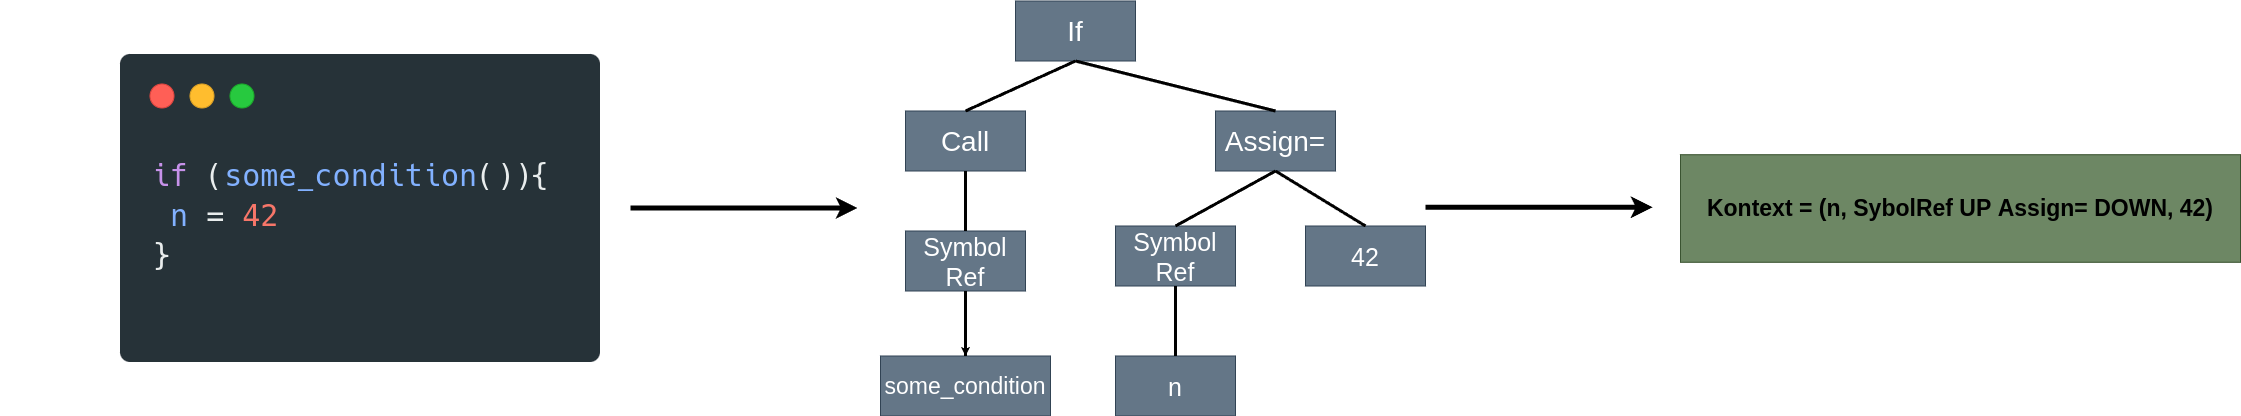
\includegraphics[scale=0.2]{abb/ast-extraction-example.drawio.png}
  \end{center}
  \caption{Die Extraktion eines Kontexts aus einem C-Quellcode}
\end{figure}
Da es unterschiedliche Konventionen für Funktionsnamen gibt, wie z.B.
\verb|Camel-Case| und \verb|Snake-Case|, normalisiert der \textit{ASTminer} 
die Funktionsnamen. Dadurch sind die Trainingsdaten unabhängig von den
jeweiligen Quellcodekonventionen.
\begin{example}
  \hfill
  \begin{center}
    Snake-Case: \verb|funktions_name| $\to$ {\bf funktions\text{\textbar}name }\\
    Camel-Case: \verb|funktionsName| $\to$ {\bf funktions\text{\textbar}name}
  \end{center}
\end{example}
Das \textit{Code2Vec}-Modell kann nach dem Training für jede 
Funktion einen hochdimensionalen
Vektor ausgeben, der den Inhalt der Funktion beschreiben soll.
Um mit \textit{Code2Vec} diesen Vektor generieren zu können, ist 
es notwendig den abstrakten Syntaxbaum als Input hinein zugegeben.
Die abstrakten Syntaxbäume können nur durch 
ihren normalisierten Namen identifiziert werden, da sie als Tupel 
in dieser Form im Datensatz vorliegen. Die normalisierten Namen
können nicht mehr 
eindeutig dem initialen Funktionsnamen zugeordnet werden, da durch die 
Normalisierung Informationen verloren gehen. Zur Vergleichbarkeit von 
\textit{Cod2Vec} mit anderen Ansätzen wie z.b. Funktionskommentaren ist
es aber wichtig,
die normalisierten Namen wieder zu den ursprünglichen Namen zurückzuführen.
Aufgrund dessen wurden im Quellcode von \textit{ASTminer} Änderungen
vorgenommen, sodass zu jeder Position eines Trainingsbeispiels im 
Datensatz der ursprüngliche Funktionsname zugeordnet werden kann. \\
\pagebreak
\hfill\\
% Code ändern bei astminer um die Namen der Funktionen am ende zuzordnen zu können
% da die Namen normalisiert werden und nicht mehr eindeutig zugeordnet werden können
% \textit{Code2Vec} erklären
Das Ziel beim Training war es, dieselbe Qualität wie Alon et al. zu erzielen. 
Das heißt, dieselben Ergebnisse für Java auch für C-Quellcode zu 
replizieren. Bei der Erstellung eines Datensatzes, der aus dem 
Modell resultiert, können bestimmte Gütekriterien beim Trainieren 
von Modellen vernachlässigt werden. Eine Problemstellung beim 
Trainieren von Modellen ist es, inwiefern das Modell generalisiert, 
also wie leistungsfähig das Modell auf neuen Daten im Gegensatz zu 
den Trainingsdaten ist.
Es ist nicht notwendig diese Problemstellung zu berücksichtigen,
da das 
Ergebnis kein fähiges Modell ist, sondern Vektoren, die den 
Inhalt der Funktion codieren.
Auch der kleine Datensatz, mit $n = 5155 $ Datenpunkten, ist zwar
für die Güte des Modells problematisch, jedoch nicht für die
resultierenden Vektoren. Selbst wenn das Modell nur 
die passenden Funktionsnamen auswendig lernt, entstehen dabei
Vektoren, die gewisse Informationen des Namens widerspiegeln.\\
Nachdem das Trainingsszenario 
genau dasselbe wie bei Alon et al. ist, wurden alle
Trainingsparameter gleich 
gelassen. Die Ergebnisse nach der 84 Epoche sind: 
{\bf Precision: $65.6$, $F_1$: $65.1$,  Recall: $64.7$}. Diese Werte sind 
etwas über den Werten von den \textit{Code2Vec} Autoren, sie kamen beim 
Full Test-Set auf: {\bf Precision: $63.1$, $F1$: $58.4$,  Recall: $54.4$}. 
Dabei ist hervorzuheben, dass unser Test- und Trainings-Datensatz derselbe ist
und der Test-Datensatz von \textit{Code2Vec} verschieden ist von dem 
Trainings-Datensatz. Die Vorgehensweise ist normalerweise grob fahrlässig,
da wir nicht die Generalisierung des Modells messen. In diesem speziellen 
Anwendungszweck ist jedoch die Güte des Modells nicht von Bedeutung,
sondern nur die Güte der erzeugten Vektoren.
Damit haben wir ähnliche Ergebnisse wie im Modell von Alon et al.
und können diese mit den anderen vorgestellten Ansätzen vergleichen
\cite{code2vec}.
%Parameterwahl und Ergebnisse
% Ganzes engeneering und pain hinter code2vec
\subsection{Funktionsnamen}
Eine andere Quellinformation, die in jedem Quellcode enthalten ist,
sind die Funktionsnamen. Funktionsnamen sollen in wenigen Wörtern 
den Kerninhalt der Funktion widerspiegeln. Dadurch eignen sich 
Funktionsnamen, um den Inhalt einer Funktion zu beschreiben. 
Die Extraktion von Funktionsnamen ist keine schwierige Aufgabe.
Hierfür wäre \textit{Tree-sitter} nicht unbedingt nötig gewesen, 
aber falls ein 
Datensatz für eine andere Sprache wie Rust erstellt werden sollte,
müsste der Parser immer wieder angepasst werden.
Deswegen wurde hier für die einfache Erweiterung des Programms,
\textit{Tree-sitter} verwendet, da \textit{Tree-sitter} Parser für 
eine Vielzahl von Sprachen anbietet.
% Motivation warum es gute semantische Vektoren erzeugen konnte
% Parsen
% Eigentlich einfach aber wenn man in Zukunft 
% Viele System nahe sprachen dazu nehmen will
% wie Rust, C, Zig, usw. 
% Ist es doch schwieriger
% -> Treesitter
%
\begin{figure}
  \begin{center}
    \begin{minipage}[c]{6cm}
        \centering
        \inputminted[fontsize=\scriptsize]{c}{comments.c}
    \end{minipage}
    \hspace{0.1cm}
    \begin{minipage}[c]{6cm}
        \centering
        \inputminted[fontsize=\scriptsize]{json}{names.json}
    \end{minipage}
  \end{center}
  \caption{Links ein Quellcode-Beispiel und rechts der extrahierte Funktionsname}
\end{figure}

\hfill\\
\pagebreak
\hfill\\

\subsection{Code-Llama-Erklärungen}
Large Language-Models werden immer besser, Quellcode selbst
zuschreiben, zu verstehen und zusammenzufassen. Eine Zusammenfassung des Quellcodes
in natürlicher Sprache spiegelt den Inhalt des Quellcodes wider.
So ist auch \textit{Code Llama} fähig, Quellcode zu erklären und
somit einen Text zu generieren, der den Inhalt der Funktion 
beschreibt. Dieser Ansatz verwendet wie \textit{Code2Vec} 
jede Quellcode-Information, da der 
gesamte Quellcode als Eingabe genutzt wird.\\
% Warum LLM's gute Embeddings produzieren könnten.
% Wir erzeugen uns eine zusammenfassung vom code
% "optimale" Kommentare
% Was ist Codellama und warum benutzten wir es?
Code Llama generiert Quellcodeerklärungen, indem Code Llama eine präzise 
Fragestellung und den gesamten Quellcode einer Funktion erhält.
Die Fragestellung (engl. prompt) ist in Abbildung 3.5 dargestellt.\\
Damit der Code-Llama-Output deterministisch ist,
ist es erforderlich, den Temperaturparameter auf null zu setzten. 
Der Parameter ist Teil einer Zufallskomponente bei der
Auswahl des nächsten Tokens, ist dieser auf null,
wird der Token mit dem höchsten Score gewählt, dieser 
bleibt bei gleicher Eingabe immer derselbe. Leider ist der
Determinismus trotzdem nicht garantiert, 
wie die Studie von Astekin et al. heraus fand
\cite{llmstable}. Laut Astekin et al. könnte ein Grund dafür sein,
dass bei den vielen Fließkommaoperationen, die für die Berechnung
eines Code-Llama-Outputs erforderlich sind,
Rundungsfehler entstehen. Diese Erkenntnisse stammen aber 
aus einem anderen Anwendungszweck, nämlich für Log-Parsing, 
geben aber ein Indiz auf eine mögliche Instabilität.\\
Die Stabilität mit Temperatur Null sollte daher für den
Anwendungszweck dieser Arbeit getestet werden. Um das zu
überprüfen, wurden von $n = ?$ Funktionen der Quellcode mit 
Fragestellung $m = ?$ Mal in Code Llama eingegeben, bei den 
resultierenden Vektoren beträgt der höchste Abstand von zwei 
Vektoren, die aus dem gleichen Quellcode resultiert sind, $d = ?$.
Dieser Abstand ist ausreichend gering, um ihn in der Evaluation 
zu vernachlässigen. Code Llama ist also für die Anwendung 
in dieser Arbeit ausreichend stabil.
\begin{figure}
  \begin{center}
    \begin{minipage}[c]{6cm}
        \centering
        \inputminted[fontsize=\small]{python}{prompt.py}
    \end{minipage}
  \end{center}
  \caption{Die verwendete Prompt für das Code-Llama-Modell }
\end{figure}
\pagebreak

\begin{figure}
  \begin{center}
    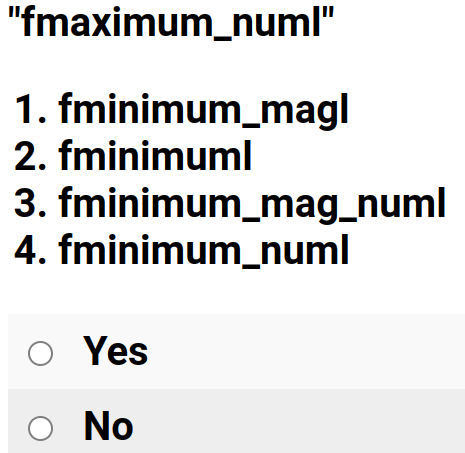
\includegraphics[scale=0.3]{abb/survey-example-positive.png}
    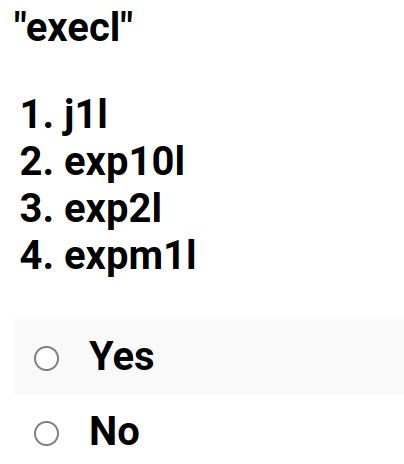
\includegraphics[scale=0.3]{abb/survey-example-negative.png}
  \end{center}
  \caption{
    Auf der linken Seite eine Frage aus dem Fragebogen die positiv
    beantwortet wurde und rechts eine Frage die negativ
    beantwortet wurde.
  }
\end{figure}

\section{Ergebnisse}
Im letzten Kapitel wurden vier verschiedene Strategien vorgestellt,
eine C-Quellcode-Funktion in einen Vektorraum abzubilden, indem 
die Vektoren den Inhalt der C-Quellcode-Funktion codieren.
Zum einen die Verwendung von Funktionsnamen und Funktionskommentaren 
die direkt aus dem C-Quellcode entnommen wurden, um diese mittels
\textit{SentenceTransformer} in Vektoren umzuwandeln. Zum anderen
aus dem gesamten C-Quellcode einer
Funktion eine Erklärung von Code Llama zu generieren, um diese 
Erklärung wieder mittels \textit{SentenceTransformer} in Embeddings
umzuwandeln. Schließlich das \textit{Code2Vec}-Modell darauf zu
trainieren,
bei gegebenem C-Quellcode einen Funktionsnamen vorherzusagen, dann 
daraus die Vektoren zu extrahieren, die für die Inferenz des Namens
bei gegebenem C-Quellcode verwendet werden.\\
Nun soll in diesem Kapitel untersucht werden, welche der vier 
Strategien
die besten Embeddings erzeugt und wie ähnlich die anderen 
Vektorräume zu dem Vektorraum der besten Strategie
sind.\\
Um diese Frage zu beantworten, welche der vorgestellten Strategien
die besten Embeddings liefern, wurde eine Expertenbefragung 
durchgeführt. Anschließend werden die erzeugten Vektorräume quantitativ
mittels einer Formel, die die Nachbarschaftsverhältnisse vergleicht, 
ausgewertet.
Zum Schluss wird qualitativ die durch \textit{t-SNE} erzeugten
zwei dimensionalen Streudiagramme verglichen.
% Vorgehensweise
% Von Chatbot zu relativ deterministischen Modell
% Ergebnisse der Standardabweichung mit Temperatur 0 \section{Ergebnisse} \subsection{Evaluierung durch Experten}
% Aufbau des Fragebogens und
% Stichproben Größe, vlt. Vorstellung der Experten
\subsection{Befragung von Experten}
Um die Befragung von Experten durchzuführen, wurde zunächst ein
Fragebogen erstellt, dafür wurde die von der 
Ludwig-Maximilians-Universität bereitgestellte Internetseite
verwendet\footnote{\url{https://survey.ifkw.lmu.de/}}. Der 
Fragebogen besteht aus $n=564 $ Fragen, wobei jede Frage aus
einer Funktion und den vier nächsten Nachbarn der Funktion im
Embedding-Raum besteht. Davon sind jeweils $k = 141$ Fragen, um
einen Embedding-Raum zu untersuchen. Also wurden, um einen
Embedding-Raum zu untersuchen, $k$ zufällige Funktionen und ihre
vier nächsten Nachbarn verwendet. Die vier Embedding-Räume
stammen aus den vier Strategien (\textit{Code2Vec}, Funktionsnamen,
Funktionskommentare und Code-Llama-Erklärungen) Embeddings zu 
erzeugen. Die Fragestellung ist nun, ob die vier nächsten Nachbarn 
der gegebenen Funktion semantisch ähnlich sind oder nicht.\\
Diese Fragen wurden dann Experten aus dem Bereich Reverse Engineering
vorgelegt. In der Abbildung 3.6 ist ein Auszug aus dem Fragebogen dargestellt.\\
Die Auswertung des Fragebogens geschah wie folgt: Jede Frage,
die positiv beantwortet wurde, gibt einen Punkt, um daraus nun 
einen Score zu berechnen werden die Punkte
summiert und dann anschließend durch die  maximal zu
erreichenden Punkte $k$ geteilt. Das Resultat ist ein normalisierter 
Score, der bei $\verb|score| = 1$ impliziert, dass alle Fragen 
positiv beantwortet wurden und bei $\verb|score| = 0$ impliziert, 
dass keine Frage positiv beantwortet wurde. Diese 
Auswertung liefert folgendes Resultat, welches in Tabelle 1
abgebildet ist.
\begin{table}
  \begin{center}
    \begin{tabular}{ |p{1.3cm}||p{3.8cm}|p{3cm}|p{1.8cm}|p{4.5cm}|  }
    \hline
    \multicolumn{5}{|c|}{Ergebnisse der Expertenbefragung} \\
    \hline
    Strategie & Funktionskommentare &  Funktionsnamen & \textit{Code2Vec} & Code-Llama-Erklärungen\\
    \hline
    Score   & 0.433 & 0.532 & 0.321 & 0.596 \\
    \hline
    \end{tabular}
  \end{center} 
  \caption{Ergebnisse der Expertenbefragung}
\end{table}
\hfill\\
Laut den Ergebnissen können die Methoden absteigend 
nach Qualität der erzeugten Embeddings folgendermaßen
angeordnet werden: \textit{Code-Llama}-Erklärungen, 
Funktionsnamen, Funktionskommentare und \textit{Code2Vec}.
Die Strategie mit dem höchsten Score ist demnach die,
die Code-Llama-Erklärungen
verwendet hat. Da nun die beste Strategie identifiziert ist, 
werden im Folgenden die anderen Strategien mit dieser quantitativ verglichen.
% Diskussion der Ergebnisse
% Folgerungen das CodeLlamma "gute" Embeddings produziert 
\pagebreak
\subsection{Quantitative Evaluierung} 
Im Folgenden wird eine Formel vorgestellt, die zwei Datenmengen
auf Ähnlichkeit untersuchen soll. Dabei ist Ähnlichkeit hier,
ähnliche Nachbarschaftsbeziehungen zu besitzen. Im Folgenden wird
eine Datenmenge als Matrix  $\mathbf{D} \in \mathbb{R}^{N\times l}$
beschrieben. Dabei ist $l \in \mathbb{N}$ die Dimension eines
Datenpunkts und $N \in \mathbb{N}$ die Anzahl der Datenpunkte. 
Folglich besitzt jeder Datenpunkt $x \in \mathbb{R}^l$ einen 
eindeutigen Index und zwar die $j$-te Zeile, für die gilt:
$x = \mathbf{D}_j$,  wobei $\mathbf{D}_j$  der $j$-te Zeilenvektor 
von $\mathbf{D}$ ist.\\ 
Zunächst wird eine Methode benötigt, um Nachbarn von einem gegebenen
Punkt zu erlangen, dafür wird hier der
\textit{K-Nearest-Neighbor-Algorithmus} verwendet. Dieser gibt bei
gegebenem Punkt die $k$ nächsten Nachbarn zurück. Also eine Funktion
mit der Signatur:
$NN_k: \mathbb{R}^{N\times l} \times \mathbb{R}^{l} \to \mathbb{N}^k$. 
Die gesamte Datenmenge und ein Datenpunkt wird eingeben und der 
Output ist ein Vektor aus Indizes, wobei jeder Index ein Nachbar 
bzw. ein Datenpunkt ist.
Diese sind aufsteigend sortiert, nach dem euklidischen Abstand 
von dem eingegebenen Punkt. Dadurch erhält man ein 
Nachbarschaftsverhältnis von einem Punkt
und seinen $k$ Nachbarn, in der Form eines Vektors
$v \in \mathbb{N}^k$.
Als Nächstes wird eine Methode benötigt, zwei 
Nachbarschaftsverhältnisse in der Form von zwei Vektoren
$u, v \in \mathbb{N}^k$ zu vergleichen.
Hierfür werden folgende Funktionen mit Signaturen
$\texttt{compare}_k:\mathbb{N}^k \times \mathbb{N}^k \to [0,1]$ 
und $\texttt{score}_k: \mathbb{N} \times \mathbb{N} \times
\mathbb{N}^k \to \{0, \frac{1}{2}, 1\}$
verwendet:
\[
    \verb|compare|(u,v)_k = 
      \frac{1}{G_k} \sum^{k}_{i=1} 
      \frac{ \texttt{score}_{k}(u_i,i,v)}{log_2(i+1)}
\]
mit
\[
  \texttt{score}_k(l,i,v) = \begin{cases*} 
      1 & , $\exists j \in \mathbb{N}: l = v_j \land i = j$   \\
      \frac{1}{2} & , $\exists j \in \mathbb{N}: l = v_j \land i \neq j$\\
      0   & , \text{otherwise}
    \end{cases*}  \text{  und  }
    G_k := \sum_{i=1}^{k} \frac{1}{log_2(i+1)}.
\]
Dabei ist die Funktion $\texttt{compare}_k$ stark durch den
Normalised Discounted Comulative Gain von Järvelin und Kekäläinen
inspiriert\cite{ndcg}.\\
Die Datenpunkte innerhalb einer Gruppierung haben zueinander einen
geringen Abstand. Aus diesem Grund ist der Score von einem
Nachbarn mit großem Abstand zum Bezugspunkt weniger bedeutsam als 
ein Nachbar mit geringem Abstand. Da die Nachbarn aufsteigend nach
Abstand zu einem gegebenen Bezugspunkt sortiert sind, wird der 
Score durch einen Wert geteilt, mit wachsenden Index größer.
Dadurch haben Nachbarn, die weiter entfernt sind, weniger Einfluss
auf die Summe. Schließlich wird noch
normalisiert, indem die höchste zu erreichende Summe an Scores
durch das Ergebnis geteilt wird. \\
Die Funktion $\texttt{score}_k$ berechnet, wie ähnlich zwei 
Nachbarschaftsverhältnisse $u, v \in \mathbb{N}^k$ bei  gegebenen
Nachbarn $l = u_i$ sind. Den  höchsten Wert 
$\texttt{score}_k(l, i, v) = 1$
bekommt ein Nachbar $l = u_i$ der im Nachbarschaftsverhältnis von $v$
enthalten ist und auf derselben Position im Abstands-Ranking von $v$
ist. 
Der Wert $\texttt{score}_k(l, i, v) = \frac{1}{2}$ bekommt ein Nachbar
$l = u_i$ der im Nachbarschaftsverhältnis $v$ enthalten ist, aber nicht auf
derselben Position im Abstands-Ranking von $v$ ist. Schließlich erhält ein 
Nachbar $l = u_i$ den Score $\text{score}_k(l, i, v) = 0$, falls er gar nicht
im Nachbarschaftsverhältnis von $v$ enthalten ist.\\
\hfill\\
\pagebreak
\hfill\\
\begin{figure}
  \begin{center}
    \begin{tikzpicture}
      \begin{axis}[
          xlabel=$k$,
          ylabel=$\text{CMP}(\mathbf{G}{,}\mathbf{D}_i{,}k)$,
          width=0.6\textwidth, 
          height=0.4\textwidth,
          legend style={nodes={scale=0.7, transform shape}}
      ]

      \addplot[ForestGreen, thick] table
        {abb/summary-embeddings-high-comment-embeddings-high-non-empty-compare.dat};
      \addplot[black, thick]
        table {abb/random-compare-plot-487x384.dat};
      \addplot[SkyBlue, thick] 
        table {abb/summary-embeddings-high-name-embeddings-high-compare487.dat};
      \addplot[CrimsonRed, thick] 
        table {abb/summary-embeddings-high-glibc-code2vec-high-compare487.dat};

      \legend{
        Funktionskommentare und Code-Llama-Erklärungen,
        Zufällige Punkte und Code-Llama-Erklärungen,
        Funktionsnamen und Code-Llama-Erklärungen,
        \textit{Code2Vec} und Code-Llama-Erklärungen
      }
      \end{axis}
    \end{tikzpicture}
  \end{center}
  \caption{
    Der Graph bildet ab, wie ähnlich verschiedene Embedding-Prozesse
    zu den Code-Llama-Erklärungen sind, für $k=2,3, \dots ,487 $, wobei
    k die Anzahl der betrachteten Nachbarn ist.
  }
\end{figure}\\
Um nun zwei Datenmengen zu vergleichen, müssen alle möglichen 
Nachbarschaftsverhältnisse betrachtet werden. Das motiviert folgende
Funktion mit Signatur:
$CMP: \mathbb{R}^{N\times l} \times  \mathbb{R}^{N\times l} \times \mathbb{N} \to [0,1]$.
Dabei wird angenommen, dass $A,B \in \mathbb{R}^{N\times l}$ Datenmengen
sind, die aus unterschiedlichen Embedding-Prozessen entstanden sind,
aber aus der gleichen Grundmenge sind. Bei einer Grundmenge $H \in F^N$,
wobei $F$ eine beliebige Menge ist und   
$E_1,E_2: F \to \mathbb{R}^{l}$ Embedding-Prozesse sind, gilt dann:
\[
  A_j = E_1(H_j)  \hspace{0.5cm }\text{und} 
  \hspace{0.5cm } B_j = E_2(H_j).
\]
Dadurch können Nachbarschaftsverhältnisse der Datenmengen $A,B$ 
verglichen werden, indem die Nachbarschaftsverhältnisse desselben 
Grundmenge in unterschiedlichen Embedding-Räumen verglichen werden:
\[
  \texttt{CMP}(A,B,k) = \frac{1}{N}\sum_{i = 1}^{N}
    \texttt{compare}_k(NN_k(A_i,A),NN_k(B_i, B))
\]
Um die Ergebnisse der $\verb|compare|_k$ Funktion zu aggregieren,
wird hier das arithmetische Mittel verwendet.
Bei den verwendeten Embedding-Prozessen in dieser Arbeit sind
Elemente der Grundmenge verloren gegangen. Die Grundmenge besteht 
hier aus den Funktionen aus der GNU-C-Standard-Bibliothek.
Die Anzahl der Vektoren in den resultierenden Datenmengen sind
deswegen verschieden: 
\[
  \verb|Funktionsnamen| \leftrightarrow \mathbf{D}_1=\mathbb{R}^{1507\times 384},
  \verb|Funktionskommentare| \leftrightarrow \mathbf{D}_2=\mathbb{R}^{487\times 384},
\]
\[
  \verb|Zufällige-Datenmenge|\leftrightarrow \mathbf{D}_3=\mathbb{R}^{1507\times 384},
  \verb|Code2Vec| \leftrightarrow \mathbf{D}_4=\mathbb{R}^{896\times 384} \hspace{0.3cm}\text{und}
\]
\[
  \hspace{0.3cm} \verb|Code-Llama-Erklärungen| \leftrightarrow \mathbf{G}=\mathbb{R}^{1507\times 384}.
\]
Um die Datenmengen vergleichen zu können, wurde das Minimum der 
Anzahl der Vektoren der verschiedenen Datenmengen genommen:
$N:= 487 = \min(1507, 487, 1507, 896, 1507) $. Da die Wahl von $k$ nicht 
offensichtlich ist, werden die Ergebnisse für alle 
$k = 2, 3, \dots, N$ berechnet und in einem 
Graphen abgebildet. Der daraus resultierende ist Graph
ist in Abbildung 4.1 dargestellt. In dem Graphen ist folgende 
Ordnung zu erkennen: 
\[ 
  \forall k=2,3,\dots,487: CMP(\mathbf{G}, \mathbf{D}_3,k) \leq 
    CMP(\mathbf{G}, \mathbf{D}_4, k) \leq 
    CMP(\mathbf{G}, \mathbf{D}_2, k) \leq 
    CMP(\mathbf{G}, \mathbf{D}_1, k)
\]
Das heißt, laut vorgestellter Formel ist der Embedding-Prozess
Funktionsnamen am ähnlichsten zu den Code-Llama-Erklärungen, 
danach Funktionskommentare, \textit{Code2Vec}-Vektoren und 
schließlich zufällige Vektoren.
% Formel um zwei Embedding spaces zu vergleichen
% Formel erklären und rechtfertigen
% Aus Umfrage rechtfertigen Codellama Summaries als gute
% embeddings zu verwenden
\begin{figure}
  \begin{center}
    \begin{tikzpicture}
      \begin{groupplot}[
            group style={
                group size=4 by 1, % 3 plots in 4 row
                horizontal sep=0.5cm, % Space between plots
                vertical sep=1cm % Space if there are multiple rows
            },
            width=0.33\textwidth, % Width of each plot
            height=0.33\textwidth, % Height of each plot 
            scatter/classes={
                0={mark=*,ContrastBlue},
                1={mark=*,ContrastRed},
                2={mark=*,ContrastGreen},
                3={mark=*,ContrastOrange},
                4={mark=*,ContrastPurple},
                5={mark=*,ContrastPink},
                6={mark=*,ContrastLime},
                7={mark=*,ContrastCyan},
                8={mark=*,Teal},
                9={mark=*,SlateGray}
            },
            scatter,
            xlabel={},
            ylabel={},
            xtick=\empty,
            ytick=\empty,
            legend style={
              at={(-1.2,-0.1)},
              legend columns=5,
              fill=none,
              draw=black,
              anchor=north,
              align=center,
              row sep=0.1cm,
              column sep=0.3cm,
              legend cell align=left
            },
        ]
          \nextgroupplot[title={\textit{Code2Vec}}]
          \addplot[scatter, only marks, scatter src=explicit symbolic]
            table[x=x, y=y, meta=label] {abb/prev-data-tsne-code2vec-tsne-30.dat};
          \nextgroupplot[title={Kommentare}]
          \addplot[scatter, only marks, scatter src=explicit symbolic]
            table[x=x, y=y, meta=label] {abb/prev-data-tsne-comment-tsne-30.dat};
          \nextgroupplot[title={Namen}]
          \addplot[scatter, only marks, scatter src=explicit symbolic]
            table[x=x, y=y, meta=label] {abb/prev-data-tsne-name-tsne-30.dat};
          \nextgroupplot[title={Code-Llama-Erklärungen}]
          \addplot[scatter, only marks, scatter src=explicit symbolic]
            table[x=x, y=y, meta=label] {abb/prev-data-tsne-summary-tsne-30.dat};
          \legend{
            IO, Netzwerk, Speicher, Nebenläufigkeit, Dateimanagement,
            Prozesse, Signale, String, Mathematik, Sonstiges
          }
        \end{groupplot}
    \end{tikzpicture}
  \end{center}
  \caption{
    Die \textit{t-SNE} Vektoren der unterschiedlichen Embedding-Prozesse
    mit Perplexity-Parameter $P = 30$.
  }
\end{figure}
\subsection{Qualitative Evaluierung} 
Die qualitative Evaluierung wird in dieser Arbeit mittels
\textit{t-SNE} durchgeführt. Dabei wird \textit{t-SNE} verwendet,
um die hochdimensionalen Vektoren $x \in \mathbb{R}^{384}$ in einen
zweidimensionalen Vektorraum zu projizieren. Bei der Verwendung und 
Interpretation von \textit{t-SNE} gibt es einiges zu beachten. \\
Zum einen sollten bei der Verwendung mehrere Werte für den
Perplexity-Parameter $P \in \{2,3,\dots ,50\}$ ausprobiert werden. 
Zum anderen kann aus den zweidimensionalen Datenmengen nur eine Aussage
über die Existenz von Clustern abgeleitet werden und nicht über die
Position und Größe einer Gruppierung. Sogar die Existenz eines Clusters 
in der zweidimensionalen Datenmenge ist zwar ein starkes Indiz,
dass ein Cluster in den hochdimensionalen Daten existiert, 
aber kein Beweis.\\
Es wurden die Werte $P \in \{20, 30, 40\}$, als Perplexity-Parameter 
verwendet, um verschiedene Werte auszuprobieren, die jeweils nicht 
am Rand der empfohlenen Menge $\{2,3, \dots, 50\}$ liegen.
Um aussagekräftige Graphen zu erhalten, wurden $1182$ Funktionen aus
der GNU-Standard-C-Bibliothek in $10$ Kategorien unterteilt. Die 
Streudiagramme mit unterschiedlichen Perplexity-Parameter sind 
jeweils im Anhang zu finden.\\
Da nun mehrere Werte für den Perplexity-Parameter ausprobiert wurden,
ohne große Unterschiede in den Gruppierungen zu erkennen, werden im 
Folgenden die vier verschiedenen Strategien, Embeddings zu erzeugen,
mit $P = 30$ abgebildet, um sie qualitativ zu vergleichen. Die 
vier Streudiagramme sind in Abbildung 4.2 dargestellt.\\
Die vier durch \textit{t-SNE} generierten Datenmengen liefern ein Indiz,
dass die Anzahl der Gruppierungen zunehmen, in der Reihenfolge: 
\textit{Cod2Vec}, Kommentare, Namen und Code-Llama-Erklärungen.
Das heißt, auch die qualitative Evaluierung scheint dem Trend zu 
folgen, dass die Qualität der Embeddings gleichermaßen aufsteigend
angeordnet ist.
% Vielleicht nochmal subsections mit Funktionsname, Funktionskommentare, 
% Funktionserklärung, und \textit{Code2Vec} Vektoren
% Probleme des jeweiligen Ansatzes mit drei Vektoren
%
\begin{figure}
  \begin{center}
    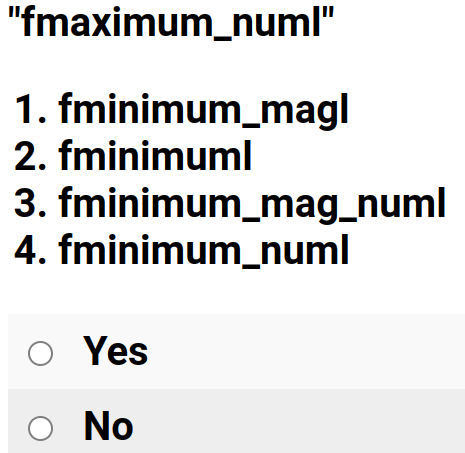
\includegraphics[scale=0.3]{abb/survey-example-positive.png}
    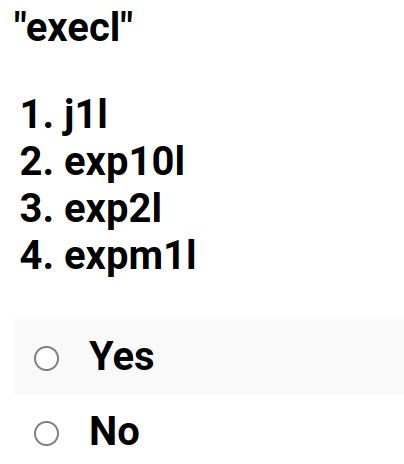
\includegraphics[scale=0.3]{abb/survey-example-negative.png}
  \end{center}
  \caption{
    Auf der linken Seite eine Frage aus dem Fragebogen die positiv
    beantwortet wurde und rechts eine Frage die negativ
    beantwortet wurde.
  }
\end{figure}
\section{Diskussion}
Das zentrale Thema dieser Arbeit, ist die semantische Ähnlichkeit
von zwei gegeben Quellcode Auszügen. Dabei ist es gar nicht so klar 
was eine gute Definition für semantische Ähnlichkeit ist.
Anhand eines Auszugs aus dem Fragebogen der in Abbildung 4.3 
dargestellt ist, ist gut zu erkennen,
was in diesen Kontext mit semantischer Ähnlichkeit gemeint ist.\\
In dem positiven Beispiel in der Abbildung 4.3, ist eine Funktion
gegeben die das Maximum von zwei Fließkommazahlen berechnet und die
vier
nächsten Nachbarn sind jeweils Variationen von Funktionen die das
Minimum von zwei Fließkommazahlen berechnen. Diese Funktionen sind
semantisch ähnlich, da sie fast äquivalente Funktionen aus dem
Mathematikmodul sind. Im negativ Beispiel der Abbildung 4.3 kreiert
die gegebene Funktionen einen neuen Prozess, dagegen haben aber die 
nächsten Nachbarn zwar einen sehr ähnlichen Namen, aber es sind 
wieder Funktionen aus dem Mathematikmodul.\\
Daher bevorzuge ich die Definition, dass zwei Funktionen semantisch
Ähnlich sind, wenn sie in ähnlichen Kontexten verwendet werden. 
Ein Beispiel hierzu wären verschiedene Sortieralgorithmen, die in 
den meisten fällen in den selben Kontexten verwendet werden können 
und damit semantisch sehr Ähnlich sind. Natürlich ist diese 
Definition nicht gerade präzise sondern sehr vage.\\
In dieser Arbeit wurden vier unterschiedliche Strategien
vorgestellt, aus C-Quellcode-Funktionen Embeddings zu erzeugen.
Die Strategien \textit{Cod2Vec}, Funktionskommentare, 
Funktionsnamen, Code-Llama-Erklärungen haben alle ihre 
eigenen Limitationen. Zunächst werden diese Problematiken
bzw. Schwächen diskutiert. Danach werden Limitationen 
und Verallgemeinerungen der $CMP$ Funktion vorgestellt.
Schließlich wird noch eine Idee für ein neues Modell 
für zukünftige Forschung beschrieben.
\pagebreak\\
\textit{Funktionsnamen}. Die Strategie, die Funktionsnamen zu 
verwenden, um Embeddings zu erzeugen, ist sehr abhängig von 
dem Quellcode. Selbst bei dem hochqualitativen Quellcode, 
der GNU-C-Standard-Bibliothek entstehen Probleme, weil die 
Namen den Inhalt der Funktion nicht präzise beschreiben.
Das folgende Problem zieht sich systematisch durch die 
ganze Bibliothek durch. In der GNU-C-Standard-Bibliothek
werden konsequent 
Abkürzungen benutzt, wodurch die Bedeutung zwar für den Mensch 
aus dem Kontext klar wird, aber wenn die Funktionsnamen 
die einzige Information ist, sind die Abkürzungen mehrdeutig.
\begin{example}
  Ein Beispiel ist die Funktion
  \verb|lchmod|. Die Funktion \verb|lchmod| passt die
  Zugriffsberechtigung einer Datei an, aber folgt dabei nicht
  symbolischen Links. Dabei werden folgende Abkürzungen verwendet:
  \begin{align*}
    \text{l} \leftrightarrow \text{link}, \hspace{0.5cm}
    \text{ch} \leftrightarrow \text{change},\hspace{0.5cm}
    \text{mod} \leftrightarrow \text{file mode}.
  \end{align*}
\end{example}
Da diese Abkürzungen nicht offensichtlich sind,
haben die durch den \textit{SentenceTransfomer} 
erzeugten Embeddings Nachbarn, welche nicht aus 
der Kategorie Dateiverwaltung sind. Die Nachbarn 
der \texttt{lchmod} Funktion im Funktionsnamen-Raum
sind: \texttt{lchmod}, \texttt{lcong48}, 
\texttt{fchmodat}, \texttt{coshl} und \texttt{cacoshl}. 
Dabei ist nur \texttt{fchmodat} aus der Kategorie 
Dateiverwaltung, diese liegt wahrscheinlich nur 
nahe an \texttt{lchmod},
da die Namen fast identisch sind. Dagegen sind die 
nächsten Nachbarn von \texttt{lchmod} im 
Code-Llama-Erklärungen-Raum alle aus der 
Kategorie Dateiverwaltung: 
\texttt{lchmod}, \texttt{fchmodat}, \texttt{fchownat},
\texttt{euidaccess} und
\texttt{\_\_file\_change\_detection\_for\_stat}.\\\\
\textit{Funktionskommentare}. 
Die Methodik der 
Funktionskommentare zu verwenden, um Embddings zu erzeugen,
ist genau wie bei den Funktionsnamen sehr abhängig von dem
Quellcode. Auch die Entscheidung, welche Kommentare man 
einbezieht, könnte Auswirkungen auf die Embeddings haben.
In dieser Arbeit wurde nur der Kommentar direkt über der 
Funktion verwendet. In zukünftiger Forschung könnte untersucht 
werden, ob die Kommentare innerhalb der Funktion auch verwendet 
werden könnten, um qualitativ hochwertigere Embeddings zu 
produzieren.\\
Auch bei den Funktionskommentaren ist das Problem, dass der 
Inhalt der Funktion sich nicht immer in dem Kommentar
widerspiegelt.
\begin{example}
  Die Funktion \verb|rand| und die Funktion \verb|rand_r| sind 
  sehr ähnlich. Erstere generiert eine zufällige Zahl im 
  Intervall $[0, \verb|RAND_MAX|]$ und zweitere generiert 
  ebenfalls eine zufällige Zahl im gleichen Intervall, aber
  erhält noch einen Seed als Parameter. Die beiden Funktionen
  haben Folgende Kommentare:
  \begin{center}
    rand $\rightsquigarrow$ Return a random integer between 0
      and RAND\_MAX.\\
    rand\_r  $\rightsquigarrow$   This algorithm is mentioned in 
    the ISO C standard, here extended for 32 bits.
  \end{center}
\end{example}
Dieses Beispiel zeigt gut, wie unterschiedlich die Qualität 
der Kommentare sein kann. Der Kommentar der Funktion \texttt{rand}
beschreibt die Funktion präzise und knapp. Dagegen verweist der 
Kommentar von der Funktion \texttt{rand\_r} nur auf einen 
ISO-C-Standard. Dadurch liefert der \textit{SentenceTransfomer}
ungenaue Ergebnisse, denn der Kosinus-Abstand zwischen
den Vektoren der Kommentare beträgt $d = 0.8544$.
Dagegen beträgt der Kosinus-Abstand von den Code-Llama-Erklärungen
der beiden Funktionen $d = 0.2216$.\\
\hfill\\
\pagebreak
\hfill\\
\textit{Code-Llama-Erklärungen.}
In dieser Arbeit wurde das größte Modell der Code-LLama-Famillie 
mit 70 Milliarden Parametern verwendet, um die 
Code-Llama-Erklärungen zu erzeugen. Aus diesem Grund ist das
gewählte Modell auch das rechenaufwendigste. In zukünftiger 
Forschung könnten kleinere Modelle mit weniger Rechenaufwand 
verwendet werden, um die Frage zu beantworten, ob der Rechenaufwand 
des Code-Llama-Modells mit 70 Milliarden Parametern nötig ist. \\
Eine weitere Problematik ist die Stabilität von Code Llama.
Bei Schwankungen von Code-Llama-Erklärungen kann nicht garantiert 
werden, dass die Erklärungen in der Praxis bei tatsächlicher 
Anwendung von gleicher Qualität sind. Deswegen sollte in
einer zukünftigen Forschung eine größere Untersuchung, 
als in dieser Arbeit, über die Stabilität von Large 
Language-Models durchgeführt werden.\\ 
Schließlich könnte in zukünftiger Forschung eine andere 
Prompt ausprobiert werden, hier könnte bspw. die 
Prompt von Wang et al. verwendet werden 
\cite{clap}. Dadurch könnten sich die Erklärungen 
verbessern und damit wieder die Qualität der 
Embeddings.\\\\
\textit{Code2Vec}. 
Diese Methodik, Embeddings zu erzeugen,
ist abhängig von der Programmiersprache des Datensatzes.  
Das \textit{Code2Vec}-Modell wurde ursprünglich für Java entwickelt,
trotzdem ist es möglich, das Modell mit anderen Programmiersprachen
zu verwenden. Für jede neue Sprache ist es erforderlich ein
Tool zu schreiben, das die besagte Sprache in das passende 
\textit{Code2Vec} Input-Format umwandelt. Außerdem ist es 
notwendig das Modell noch zu trainieren, um danach bei 
gegebener Funktion einen Vektor zu produzieren. Deswegen 
kann je nach Datensatz der Aufwand,
um die Embeddings zu generieren, hoch sein. \\
Eine weitere Schwäche ist die Abhängigkeit von der Namensgebung 
der Funktionen im Datensatz, da das \textit{Code2Vec} Modell 
darauf trainiert wird, Funktionsnamen vorherzusagen, dadurch 
enstehen dieselben Probleme wie bei der Diskussion zu 
den Funktionsnamen.\\
Des Weiteren könnten die bescheidenen Ergebnisse des 
\textit{Code2Vec}-Modells anhand der Sprache des Datensatzes,
der Qualität der Funktionsnamen im Datensatz oder auch durch die 
Größe des Datensatzes erklärt werden.\\\\
\textit{Die \texttt{CMP} Funktion.} 
In dieser Arbeit wurde die \texttt{CMP}-Funktion vorgestellt, welche 
zwei Datenmengen anhand ihrer Nachbarschaftsbeziehungen vergleicht.
Sie berechnet für zwei Datenmengen $A,B \in \mathbb{R}^{N\times l}$
einen Ähnlichkeit-Score 
$\texttt{CMP}(A,B,k) = s \in [0,1]\subset \mathbb{R}$.
Dabei ist $N$ die Größe der Datenmengen, $l$ die Dimension der 
Vektoren in der Datenmenge und k die Anzahl der Nachbarn, 
die verglichen werden sollen. Analog zum Perplexity-Parameter
bei \textit{t-SNE}, sollte $k$ nach der Größe der Gruppierungen 
in den Datenmengen gewählt werden. Dabei reagiert die Formel 
wesentlich empfindlicher auf Änderungen von $k$, als der 
Perplexity-Parameter in \textit{t-SNE}. In zukünftiger Forschung 
könnte ein Intervall herausgearbeitet werden $a \le k \le b $ mit
$ a,b \in \mathbb{N}$ oder sogar einen  optimalen Wert 
$k := C\in \mathbb{N}$ für alle Datenmengen.
Das ist auch wünschenswert, da die Formel für 
alle $k = 2,3,\dots, N$ auszurechnen einen hohen Rechenaufwand 
darstellt. Das liegt primär an dem K-Nearest-Neighbor-Algorithmus 
bzw. an einer Funktion, die Nachbarn aufsteigend sortiert nach 
dem Abstand zu eingegebenen Punkt berechnet. Die restlichen 
Operationen sind elementare Rechenoperationen. Zunächst könnte 
man also verschiedene Funktionen ausprobieren, die die Nachbarn 
aufsteigend nach dem Abstand zum eingegebenen Punkt sortiert.
\hfill\\
\pagebreak
\hfill\\
Das liefert folgende Verallgemeinerung:
\[
  \text{Sei  }f_k \in \{\mathbb{R}^{N\times l}
  \times \mathbb{R}^l \to \mathbb{N}^k\} 
  \text{ beliebig, mit oben beschriebenen Eigenschaften, dann gilt:}
\]

\[
  CMP(A,B,k) = 
  \frac{1}{N}\sum_{i = 1}^{N} 
  \verb|compare|_k(f_k(A_i,A),f_k(B_i, B)).
\]
Des Weiteren wurde hier, um die Resultate der Funktion 
$\verb|compare|_k$ zu aggregieren, das arithmetische Mittel
verwendet. Diese Wahl ist willkürlich und könnte durch eine 
andere Aggregationsmethode ersetzt werden. Daraus
folgt die nächste Verallgemeinerung:
\begin{center}
  Sei $f_k \in \{\mathbb{R}^{N\times l}
  \times \mathbb{R}^l \to \mathbb{N}^k\}$ wie oben und 
  $agg \in \{\mathcal{P}([0,1]) \to [0,1]\}$ beliebig, 
  dann gilt:
\end{center}
\[ 
  CMP(A,B,k) = 
  agg(\{\verb|compare|_k(f_k(A_i,A),f_k(B_i,B)) 
    \hspace{0.1cm}|\hspace{0.1cm} i = 1,2, \dots N\})
\]
Die letzte Verallgemeinerung betrifft die $\verb|score|_k$
Funktion. 
\[
  \text{score}_k(l,i,v) = \begin{cases*} 
      1 & , $\exists j \in \mathbb{N}: l = v_j \land i = j$   \\
      \frac{1}{2} & , $\exists j \in \mathbb{N}: l = v_j \land i \neq j$\\
      0   & , \text{otherwise}
    \end{cases*}  \text{  und  }
    G_k := \sum_{i=1}^{k} \frac{1}{log_2(i+1)}.
\]
Der Wert, den die Funktion zurückgibt, wenn der Nachbarindex 
$l$ in dem Nachbarschaftsverhältnis $v$ enthalten ist,
aber nicht auf derselben Position ist,
beträgt $\verb|score|_k(l,i,v) = \frac{1}{2}$. 
Dieser ist wiederum völlig willkürlich gewählt.
Deswegen wäre hier eine sinnvolle Verallgemeinerung:
\begin{center}
  Sei $a \in (0,1) \subset \mathbb{R}$ beliebig, dann gilt:
\end{center}
\[
  \text{score}_k(l,i,v) = \begin{cases*} 
      1 & , $\exists j \in \mathbb{N}: l = v_j \land i = j$   \\
      a & , $\exists j \in \mathbb{N}: l = v_j \land i \neq j$\\
      0 & , \text{otherwise}
    \end{cases*}  \text{  und  }
    G_k := \sum_{i=1}^{k} \frac{1}{log_2(i+1)}.
\]
All diese Verallgemeinerungen motivieren das
Ausprobieren verschiedener Instanzen der verallgemeinerten 
Objekte. In zukünftiger Forschung könnte herausgefunden  
werden, welche Vorteile und Nachteile, die verschiedene 
Instanzen haben.\\\\
\textit{Code2Vec und BERT als Inspiration für ein neues Modell.} 
Nach meiner Meinung ist das größte Problem von \textit{Code2Vec} 
die Abhängigkeit von den Funktionsnamen der Trainingsdaten und 
das überwachte Lernen. Anstatt das Modell darauf zu trainieren,
Funktionsnamen vorherzusagen, könnte man mit unüberwachten Lernen,
wie in dem BERT-Modell, Trainingsaufgaben geben, welche das 
Verständnis von Quellcode stärken. Da der Input von 
\textit{Code2Vec} ein abstrakter Syntaxbaum ist, könnte hier eine 
Aufgabe sein, ein fehlenden Knoten im Baum vorherzusagen. Eine 
weitere Trainingsaufgabe könnte sein, ob zwei Zweige in 
einem abstrakten Syntaxbaum sequenziell hintereinander kommen oder 
nicht. Dazu könnte man entweder noch das Prinzip von Aufmerksamkeit
aus der Transformer-Architektur oder \textit{Code2Vec} übernehmen.
%copy Evaluation
% Zusammenfassung der jeweiligen Resultate
% Funktionnamen -> Nicht geignet, da zu wenig informationen und abkürzungen
% Funktionskommentare -> Je nach Projekt geignet, aber nicht allgemeingültig
%     deswegen eher ungeignet
% \textit{Code2Vec} -> Kommt nur knapp an mit benutzuten Daten an Names ran also nicht 
% geignet
\pagebreak
\section{Fazit}
In dieser Arbeit wurden vier verschiedene Arten vorgestellt,
aus C Quellcode reellwertige Vektoren zu produzieren, die den 
Inhalt der Funktion codieren. Zum einen wurden aus Funktionsnamen, 
Funktionskommentaren und Code-Llama-Erklärrungen, mittels 
\textit{SentenceTransfomer}, Vektoren produziert.
Zum anderen wurden aus dem \textit{Code2Vec} Modell, welches
auf C adaptiert wurde, die Inferenz-Vektoren entnommen.\\
Durch eine Expertenbefragung konnte die besten Embeddings
identifiziert werden, diese sind aus den Code-Llama-Erklärungen
entstanden. Des Weiteren wurde eine quantitative Auswertung 
durchgeführt, mittels einer Funktion, die eine Datenmengen
mit den Code-Llama-Vektoren anhand ihrer 
Nachbarschaftsbeziehungen vergleicht.
Schließlich wurde eine qualitative Evaluierung durchgeführt 
indem die verschiedenen Embedding-Prozesse durch \textit{t-SNE}
in die 2-dimensionalen Ebene projiziert wurde, um diese
auf Gruppierungen zu untersuchen. 
Dabei resultierte, dass die Code-Llama-Erklärungen die 
Embeddings mit der höchsten Qualität produzieren.
Diese sind gefolgt von Funktionsnamen, danach Funktionskommentare 
und schließlich \textit{Code2Vec}.
Wobei im Allgemeinen nicht offensichtlich ist, was ein 
hochqualitatives Embedding ist, da wiederum nicht klar ist,
wie man die semantische Ähnlichkeit zwischen zwei 
Quellcodeabschnitten Formal definiert.\\
Die von den Code-Llama-Erklärungen erzeugten Vektoren
könnten direkt eingesetzt werden, um viele verschiedene
Problemstellungen für die C-Programmiersprache zu lösen.\\
Die Motivation dieser Arbeit war es aber Vektoren für 
Neuronales Netzwerk zu generieren, um dieses neuronale Netzwerk,
mittels überwachten Lernens darauf zu trainieren, bei gegebener
Funktion in Maschinensprache einen Vektor vorherzusagen, der den
Inhalt der Funktion codiert.
Die resultierenden Vektoren, die den Inhalt des Binärcodes codieren,
können dann benutzt werden, um neuronale Netzwerke auf diverse
Anwendungen zu trainieren, wie Beispielsweise
\textit{Binary Code-Similarity-Detection} \cite{jtrans},
\textit{Function-Boundary-Detection} \cite{190918},
\textit{Function-Type-Inference}\cite{203650},
\textit{Binary Code-Search} \cite{9345532},
Reverse Engineering \cite{reverse-engeneering},
oder das Klassifizieren von 
Maleware in der Maschinensprache\cite{maleware-detection}. 
Dieses Neuronales Netzwerk könnte nun mit den Vektoren,
welche aus den Code-Llama-Erklärungen erzeugt wurden,
trainiert werden.




\pagebreak

\appendix
\section{t-SNE Graphen}
\begin{figure}[H]
  \begin{center}
    \begin{tikzpicture}
      \begin{groupplot}[
            group style={
                group size=3 by 1,
                horizontal sep=0.5cm, % Space between plots
                vertical sep=1cm % Space if there are multiple rows
            },
            width=0.33\textwidth, % Width of each plot
            height=0.33\textwidth, % Height of each plot 
            scatter/classes={
                0={mark=*,ContrastBlue},
                1={mark=*,ContrastRed},
                2={mark=*,ContrastGreen},
                3={mark=*,ContrastOrange},
                4={mark=*,ContrastPurple},
                5={mark=*,ContrastPink},
                6={mark=*,ContrastLime},
                7={mark=*,ContrastCyan},
                8={mark=*,Teal},
                9={mark=*,SlateGray}
            },
            scatter,
            xlabel={},
            ylabel={},
            xtick=\empty,
            ytick=\empty,
            legend style={
              at={(-0.6,-0.1)},
              legend columns=5,
              fill=none,
              draw=black,
              anchor=north,
              align=center,
              row sep=0.1cm,
              column sep=0.3cm,
              legend cell align=left
            },
        ]
          \nextgroupplot[title={\textit{Code2Vec}, $P=20$}]
          \addplot[scatter, only marks, scatter src=explicit symbolic]
            table[x=x, y=y, meta=label] {abb/prev-data-tsne-code2vec-tsne-20.dat};
          \nextgroupplot[title={\textit{Code2Vec}, $P=30$}]
          \addplot[scatter, only marks, scatter src=explicit symbolic]
            table[x=x, y=y, meta=label] {abb/prev-data-tsne-code2vec-tsne-30.dat};
          \nextgroupplot[title={\textit{Code2Vec}, $P=40$}]
          \addplot[scatter, only marks, scatter src=explicit symbolic]
            table[x=x, y=y, meta=label] {abb/prev-data-tsne-code2vec-tsne-40.dat};

          \legend{
            IO, Netzwerk, Speicher, Nebenläufigkeit, Dateimanagement,
            Prozesse, Signale, String, Mathematik, Sonstiges
          }
        \end{groupplot}
    \end{tikzpicture}
  \end{center}
  \caption{
    Die \textit{t-SNE} Vektoren, mit unterschiedlichen Perplexity-Parameter,
    produziert aus den hochdimensionalen
    \textit{Code2Vec} Vektoren. Die Grafik liefert bei jedem der 
    Perplexity-Parameter ein Indiz dafür, dass die 
    Mathematik- und IO-Funktionen jeweils größtenteils in den 
    hochdimensionalen Daten ein Cluster bilden. Sonst ist keine weitere
    Gruppierung zu erkennen.
  }
\end{figure}
\begin{figure}[H]
  \begin{center}
    \begin{tikzpicture}
      \begin{groupplot}[
            group style={
                group size=3 by 1,
                horizontal sep=0.5cm, % Space between plots
                vertical sep=1cm % Space if there are multiple rows
            },
            width=0.33\textwidth, % Width of each plot
            height=0.33\textwidth, % Height of each plot 
            scatter/classes={
                0={mark=*,ContrastBlue},
                1={mark=*,ContrastRed},
                2={mark=*,ContrastGreen},
                3={mark=*,ContrastOrange},
                4={mark=*,ContrastPurple},
                5={mark=*,ContrastPink},
                6={mark=*,ContrastLime},
                7={mark=*,ContrastCyan},
                8={mark=*,Teal},
                9={mark=*,SlateGray}
            },
            scatter,
            xlabel={},
            ylabel={},
            xtick=\empty,
            ytick=\empty,
            legend style={
              at={(-0.6,-0.1)},
              legend columns=5,
              fill=none,
              draw=black,
              anchor=north,
              align=center,
              row sep=0.1cm,
              column sep=0.3cm,
              legend cell align=left
            },
        ]
          \nextgroupplot[title={Kommentare, $P=20$}]
          \addplot[scatter, only marks, scatter src=explicit symbolic]
            table[x=x, y=y, meta=label] {abb/prev-data-tsne-comment-tsne-20.dat};
          \nextgroupplot[title={Kommentare, $P=30$}]
          \addplot[scatter, only marks, scatter src=explicit symbolic]
            table[x=x, y=y, meta=label] {abb/prev-data-tsne-comment-tsne-30.dat};
          \nextgroupplot[title={Kommentare, $P=40$}]
          \addplot[scatter, only marks, scatter src=explicit symbolic]
            table[x=x, y=y, meta=label] {abb/prev-data-tsne-comment-tsne-40.dat};

          \legend{
            IO, Netzwerk, Speicher, Nebenläufigkeit, Dateimanagement,
            Prozesse, Signale, String, Mathematik, Sonstiges
          }

        \end{groupplot}
    \end{tikzpicture}
  \end{center}
  \caption{
    Die \textit{t-SNE} Vektoren, mit unterschiedlichen Perplexity-Parameter,
    produziert aus den hochdimensionalen
    Funktionskommentar-Embeddings. Hier gibt es, wie im vorherigen Abschnitt
    beschrieben, deutlich weniger Punkte als bei den restlichen Strategien,
    Embeddings zu erzeugen. 
    In den drei Graphen ist eine große Gruppierung in der Kategorie
    Dateimanagement und kleine Gruppierungen in den Kategorien Mathematik,
    String und Signale zu erkennen.
  }
\end{figure}
\begin{figure}[H]
  \begin{center}
    \begin{tikzpicture}
      \begin{groupplot}[
            group style={
                group size=3 by 1,
                horizontal sep=0.5cm, % Space between plots
                vertical sep=1cm % Space if there are multiple rows
            },
            width=0.33\textwidth, % Width of each plot
            height=0.33\textwidth, % Height of each plot 
            scatter/classes={
                0={mark=*,ContrastBlue},
                1={mark=*,ContrastRed},
                2={mark=*,ContrastGreen},
                3={mark=*,ContrastOrange},
                4={mark=*,ContrastPurple},
                5={mark=*,ContrastPink},
                6={mark=*,ContrastLime},
                7={mark=*,ContrastCyan},
                8={mark=*,Teal},
                9={mark=*,SlateGray}
            },
            scatter,
            xlabel={},
            ylabel={},
            xtick=\empty,
            ytick=\empty,
            legend style={
              at={(-0.6,-0.1)},
              legend columns=5,
              fill=none,
              draw=black,
              anchor=north,
              align=center,
              row sep=0.1cm,
              column sep=0.3cm,
              legend cell align=left
            },
        ]
          \nextgroupplot[title={Namen, $P=20$}]
          \addplot[scatter, only marks, scatter src=explicit symbolic]
            table[x=x, y=y, meta=label] {abb/prev-data-tsne-name-tsne-20.dat};
          \nextgroupplot[title={Namen, $P=30$}]
          \addplot[scatter, only marks, scatter src=explicit symbolic]
            table[x=x, y=y, meta=label] {abb/prev-data-tsne-name-tsne-30.dat};
          \nextgroupplot[title={Namen, $P=40$}]
          \addplot[scatter, only marks, scatter src=explicit symbolic]
            table[x=x, y=y, meta=label] {abb/prev-data-tsne-name-tsne-40.dat};

          \legend{
            IO, Netzwerk, Speicher, Nebenläufigkeit, Dateimanagement,
            Prozesse, Signale, String, Mathematik, Sonstiges
          }
        \end{groupplot}
    \end{tikzpicture}
  \end{center}
    \caption{
      Die \textit{t-SNE} Vektoren, mit unterschiedlichen 
      Perplexity-Parameter, produziert aus den hochdimensionalen
      Funktionsnamen-Embeddings. In der Abbildung ist zu erkennen, 
      dass die Kategorien Nebenläufigkeit, Speicher, Mathematik und
      Signale eine Gruppierung bilden. Dagegen teilen sich die Kategorien
      Netzwerk, IO, String in mehrere Untergruppierungen auf.
    }
\end{figure}
\begin{figure}[H]
  \begin{center}
    \begin{tikzpicture}
      \begin{groupplot}[
            group style={
                group size=3 by 1,
                horizontal sep=0.5cm, % Space between plots
                vertical sep=1cm % Space if there are multiple rows
            },
            width=0.33\textwidth, % Width of each plot
            height=0.33\textwidth, % Height of each plot 
            scatter/classes={
                0={mark=*,ContrastBlue},
                1={mark=*,ContrastRed},
                2={mark=*,ContrastGreen},
                3={mark=*,ContrastOrange},
                4={mark=*,ContrastPurple},
                5={mark=*,ContrastPink},
                6={mark=*,ContrastLime},
                7={mark=*,ContrastCyan},
                8={mark=*,Teal},
                9={mark=*,SlateGray}
            },
            scatter,
            xlabel={},
            ylabel={},
            xtick=\empty,
            ytick=\empty,
            legend style={
              at={(-0.6,-0.1)},
              legend columns=5,
              fill=none,
              draw=black,
              anchor=north,
              align=center,
              row sep=0.1cm,
              column sep=0.3cm,
              legend cell align=left
            },
        ]
          \nextgroupplot[title={\textit{Code Llama}, $P=20$}]
          \addplot[scatter, only marks, scatter src=explicit symbolic]
            table[x=x, y=y, meta=label] {abb/prev-data-tsne-summary-tsne-20.dat};
          \nextgroupplot[title={\textit{Code Llama}, $P=30$}]
          \addplot[scatter, only marks, scatter src=explicit symbolic]
            table[x=x, y=y, meta=label] {abb/prev-data-tsne-summary-tsne-30.dat};
          \nextgroupplot[title={\textit{Code Llama}, $P=40$}]
          \addplot[scatter, only marks, scatter src=explicit symbolic]
            table[x=x, y=y, meta=label] {abb/prev-data-tsne-summary-tsne-40.dat};

          \legend{
            IO, Netzwerk, Speicher, Nebenläufigkeit, Dateimanagement,
            Prozesse, Signale, String, Mathematik, Sonstiges
          }
        \end{groupplot}
    \end{tikzpicture}
  \end{center}
  \caption{
    Die \textit{t-SNE} Vektoren, mit unterschiedlichen Perplexity-Parameter,
    produziert aus den hochdimensionalen Code-Llama-Erklärungen-Embeddings.
    In der Abbildung ist zu erkennen, dass die Kategorien Nebenläufigkeit,
    Speicher, Mathematik und Signale eine Gruppierung bilden. Dagegen 
    teilen sich die Kategorien Netzwerk, IO, String in mehrere 
    Untergruppierungen auf.
  }
\end{figure}\hfill\\

\pagebreak

\addcontentsline{toc}{section}{Literatur}
%\pagestyle{fancy}

\bibliographystyle{IEEEtran}
\bibliography{bibliography} %bib-filename

\nocite{*} %List all bib-entries

\end{document}
